\documentclass[10pt, letterpaper]{article}

\usepackage{setspace}
\usepackage[letterpaper, margin=1.0in]{geometry}
%\usepackage{lscape}
\usepackage{amsmath}   % includes \boldmath(), \boldsymbol{()}
\usepackage{bm}        % math fonts, \boldmath{}, \boldsymbol{}
\usepackage[authoryear, round, semicolon]{natbib}
\bibliographystyle{plainnat}
%\usepackage[style=apa, citestyle=authoryear, language=american]{biblatex}
%\DeclareLanguageMapping{american}{american-apa}
%\addbibresource{XTXBibliography.bib}
%\bibliographystyle{plain}
%\renewcommand\multicitedelim{\addsemicolon\space}
\usepackage{graphicx}
\graphicspath{ {Images/} }
\usepackage{float}
\usepackage{caption}
\captionsetup[table]{skip=10pt, belowskip=12pt}
\providecommand{\keywords}[1]{\noindent\textbf{Keywords:  } #1}
\usepackage{subcaption}
\newcommand{\mt}[1]{\bm{#1}^{\prime}}
\newcommand{\mtm}[2]{\bm{#1}^{\prime}\bm{#2}}
\newcommand{\mi}[1]{\bm{#1}^{-1}}
\newcommand{\mest}[1]{\hat{\bm{#1}}}
\usepackage[bottom]{footmisc}
\setlength{\skip\footins}{12pt}
\setlength\parindent{0pt}

\begin{document}

\begin{spacing}{1.0}

Duke University Synthetic Data Project
    
Threshold Verification Measure

Simulated Threshold Measure Distribution as a Function of Number of Partitions and Epsilon

Race Disparity Fixed Effects Model using Small to Large Agency, Occupation Subsets

2/18/2018, T. Balmat

\vspace{20pt}

In computing the threshold verification measure for regression models using agency, occupation, and sex subsets of authentic OPM data, subset observations are partitioned such that a uniform number of employees are represented in each partition and each employee appears in one partition only.  A common model is fit to each partition and the proportion of partitions with parameter of interest having an estimate beyond the specified threshold value is reported, after application of privacy protecting statistical noise.  A model to estimate within agency, occupation, and sex pay disparity by race is

\vspace{-24pt}
\begin{center}
    \begin{equation}
    y=\beta_0 + \beta_{race} + \beta_{age} \times age + \beta_{age^2} \times + age^2 + \beta_{ed} \times ed_{years} + \beta_{year}
    \label{model:OPM-lnPay-Race}
    \end{equation}
\end{center}

where $y$ is the logarithm of \textit{basic pay} and \textit{race}, \textit{sex}, \textit{age}, \textit{education}, and \textit{year} are independent covariates.  \textit{year} is used as controlling fixed effect.  To assess interaction of \textit{sex} and \textit{race}, comparison of corresponding race coefficients computed from female and male subsets is made. 

\vspace{12pt}

[\textit{Purpose of study}]\\

[\textit{Description of data and source}]\\

In order to assess the effect of partition count and number of observations per partition, small to large subsets of authentic observations for distinct combinations of agency, occupation, sex, and race were chosen.  These appear in table \ref{table:AgencyOcc}.  In addition to possessing the desired range of observation counts, the race coefficient estimates produced from fitting model (\ref{model:OPM-lnPay-Race}) to the subsets are at distances from the important policy threshold value of -0.01 that demonstrate strengths and weaknesses of the threshold verification method.\footnote{Explain or reference threshold measure and origin of -0.01 policy value}

\begin{table}[h!]
    \centering
    \caption{Large to small authentic observation agency, occupation, sex and race subsets chosen for simulation.}
    \begin{tabular}{llllr}
      \hline
      Agency & & Occupation & & Total Observations \\ 
      \hline\\[-6pt]
      VATA & Veterans Health Admin & 620 & Practical Nurse & 66,394 \\
      SZ00 & Social Security Admin & 105 & Insurance Admin & 42,709 \\
      TD03 & Federal Aviation Admin & 2152 & Air Traffic Ctl & 21,416 \\
      TR93 & Internal Revenue Serv & 592 & Tax Examining & 3,963 \\ 
      DJ09 & Off of US Attorney & 0905 & Gen Attorney & 3,748 \\
      DJ02 & FBI & 1811 & Criminal Investigating & 1,225 \\
      LF00 & Fed Elec Comm & 0905 & Gen Attorney & 32 \\
      \hline
    \end{tabular}
    \label{table:AgencyOcc}
\end{table}

\clearpage

\begin{table}
    \begin{tabular}{p{1in}p{5in}}
    Definitions & \\
    \hline
    & \\    
    Partition: &  A subset of observations from the entire data set such that for each pseudo (employee) ID appearing in contained observations, no observations for the pseudo ID appear in another partition.  Pseudo IDs are randomly and uniformly distributed to partitions.  Note that, since employees can have different numbers of observations, actual partition sizes (number of observations) can vary.\\
    & \\[-6pt]
    Threshold value: & Fixed value, specified by analyst, used to count number of partitions with estimated coefficient at or beyond (below in this study).\\
    & \\[-6pt]
    M: & The number of partitions to create from the entire agency, occupation, and sex sub set.\\
    & \\[-6pt]
    S: & S is the number, of the M partitions, that have coefficient of interest, computed from fitting model (\ref{model:OPM-lnPay-Race}), at or beyond the threshold value.  If, due to dependencies among independent variables or lack of observations for a factor (race) level of interest, the model cannot be fit to all M partitions then S is computed as the prorated number of partitions of M corresponding to the ratio of number of partitions at or beyond threshold to partitions with computable coefficients.\\
    & \\[-6pt]
    Posterior p & Proportion partitions at or beyond threshold, adjusted using statistical algorithm to apply privacy protecting noise.\footnote{Reference posterior p algorithm}\\
    & \\[-6pt]
    $\epsilon$: & The privacy protecting parameter of the posterior p algorithm.\footnote{Reference $\epsilon$ in posterior p algorithm}\\
    
    \end{tabular}
\end{table}

\vspace{20pt}

Simulation\\[-8pt]
\noindent\rule{\textwidth}{0.5pt}\\[-6.25pt]

Subsets of authentic OPM observations for combinations of agency, occupation, and sex listed in table \ref{table:AgencyOcc} were uniformly divided into disjoint-pseudo ID partitions and model (\ref{model:OPM-lnPay-Race}) was fit to each partition.  Using race E (white) as reference level, computed coefficients for races indicated in table \ref{table:AgencyOcc} were used as inputs to the posterior p algorithm, along with values for the privacy protecting parameter $\epsilon$.\footnote{OPM Race codes are A (Native American), B (Asian), C (black), and D (Hispanic), and E(white).}  This was repeated ten times, each time using five levels of M and three levels of $\epsilon$.  Values for actual proportion partitions at threshold and posterior noise induced values of proportion at threshold were recorded.  Since the verification process is intended to confirm actual covariate relationships in authentic and synthetic data, it is useful to report these for reference.  Table \ref{table:CoefficientFullSet} lists, for each complete (non-partitioned) set of observations, coefficients computed using authentic data ($\beta_\text{auth}$), along with associated standard errors, number of observations in the agency, occupation, sex subset that the model was fit to (recall that there exist observations for multiple races), the number of observations for the race subset, and the coefficient estimate obtained from fitting the model to the corresponding synthetic data subset ($\beta_\text{synth}$).

\begin{table}[h]
    \centering
    \caption{Computed race coefficients using complete (non-partitioned) subsets for indicated agency, occupation, sex, and race.}
    \begin{tabular}{rllllrrrrr}
        \hline\\[-10pt]
        & Agency & Occupation & Sex & Race & $\mest{\beta}_\text{auth}$ & SE & n(Agency-Occ-Sex) & n(Race) & $\mest{\beta}_\text{synth}$ \\ 
        \hline\\[-6pt]
        1 & VATA & 620 & F & Race(C) & 0.02 & 0.0007 & 193,144 & 66,394 & 0.03 \\ 
        2 & SZ00 & 105 & F & Race(D) & -0.04 & 0.0010 & 305,311 & 42,709 & -0.04 \\ 
        3 & TD03 & 2152 & M & Race(C) & -0.05 & 0.0018 & 458,114 & 21,416 & -0.06 \\ 
        4 & TR93 & 592 & F & Race(B) & -0.03 & 0.0023 & 165,210 & 3,963 & -0.04 \\ 
        5 & DJ09 & 905 & F & Race(C) & -0.01 & 0.0027 & 34,154 & 3,748 & -0.01 \\ 
        6 & DJ02 & 1811 & F & Race(B) & -0.04 & 0.0046 & 42,077 & 1,225 & -0.06 \\ 
        7 & LF00 & 905 & F & Race(B) & -0.05 & 0.0329 & 705 & 32 & -0.06 \\ 
        \hline
    \end{tabular}
    \label{table:CoefficientFullSet}
\end{table}

\vspace{20pt}

Tables \ref{table:Coefficient-M=10}, \ref{table:Coefficient-M=30}, and \ref{table:Coefficient-M=50} report summarized results of the ten iterations of partitioning and posterior p computation for partition sizes M = 10, 30 , and 50 and $\epsilon$ values of 0.5, 1, and 2.  Rows of these tables correspond to like numbered rows of table \ref{table:CoefficientFullSet}.  The ``Observed p" columns contain mean proportion partitions at threshold for all iterations and the ``p" columns contain mean computed posterior p for all iterations using the indicated value of $\epsilon$.  Of note is that, for each M, agreement of mean posterior p with corresponding mean observed p improves with increase in $\epsilon$.  This is consistent with the role of $\epsilon$ in protecting privacy.\footnote{cite}  There does not appear to be any significant degradation in mean posterior p with decrease in partition size (recall that observation counts decrease for increasing row numbers).

\begin{table}[h]
    \centering
    \caption{Posterior p results for number of partitions M = 10 and $\epsilon$ = 0.5, 1, and 2.  Values are the mean results of ten iterations.  Row IDs correspond with table \ref{table:CoefficientFullSet}.}
    \begin{tabular}{rlrrrr}
        \hline\\[-10pt]
        & Subset & Observed p & p($\epsilon$=0.5) & p($\epsilon$=1) & p($\epsilon$=2) \\ 
        \hline\\-6pt]
        1 & VATA-620-F-C & 0.00 & 0.13 & 0.01 & 0.02 \\ 
        2 & SZ00-105-F-D & 1.00 & 0.87 & 0.92 & 0.97 \\ 
        3 & TD03-2152-M-C & 1.00 & 0.82 & 0.88 & 0.96 \\ 
        4 & TR93-592-F-B & 0.92 & 0.79 & 0.91 & 0.93 \\ 
        5 & DJ09-905-F-C & 0.44 & 0.41 & 0.40 & 0.46 \\ 
        6 & DJ02-1811-F-B & 0.87 & 0.90 & 0.83 & 0.86 \\ 
        7 & LF00-905-F-B & 0.67 & 0.67 & 0.74 & 0.69 \\ 
        \hline
    \end{tabular}
    \label{table:Coefficient-M=10}
\end{table}

\begin{table}[h]
    \centering
    \caption{Posterior p results for number of partitions M = 30 and $\epsilon$ = 0.5, 1, and 2.  Values are the mean results of ten iterations.  Row IDs correspond with table \ref{table:CoefficientFullSet}.}
    \begin{tabular}{rlrrrr}
        \hline\\[-10pt]
        & Subset & Observed p & p($\epsilon$=0.5) & p($\epsilon$=1) & p($\epsilon$=2) \\ 
        \hline\\[-6pt]
        1 & VATA-620-F-C & 0.00 & 0.04 & 0.03 & 0.01 \\ 
        2 & SZ00-105-F-D & 0.99 & 0.98 & 0.97 & 0.98 \\ 
        3 & TD03-2152-M-C & 0.92 & 0.96 & 0.92 & 0.92 \\ 
        4 & TR93-592-F-B & 0.80 & 0.79 & 0.81 & 0.80 \\ 
        5 & DJ09-905-F-C & 0.47 & 0.50 & 0.47 & 0.46 \\ 
        6 & DJ02-1811-F-B & 0.73 & 0.74 & 0.76 & 0.74 \\ 
        7 & LF00-905-F-B & 0.54 & 0.54 & 0.53 & 0.54 \\ 
        \hline
    \end{tabular}
    \label{table:Coefficient-M=30}
\end{table}

\begin{table}[ht]
    \centering
    \caption{Posterior p results for number of partitions M = 50 and $\epsilon$ = 0.5, 1, and 2.  Values are the mean results of ten iterations.  Row IDs correspond with table \ref{table:CoefficientFullSet}.}
    \begin{tabular}{rlrrrr}
        \hline\\[-10pt]
        & Subset & Observed p & p($\epsilon$=0.5) & p($\epsilon$=1) & p($\epsilon$=2) \\ 
        \hline\\[-6pt]
        1 & VATA-620-F-C & 0.00 & 0.04 & 0.02 & 0.01 \\ 
        2 & SZ00-105-F-D & 0.96 & 0.94 & 0.96 & 0.96 \\ 
        3 & TD03-2152-M-C & 0.85 & 0.87 & 0.85 & 0.84 \\ 
        4 & TR93-592-F-B & 0.73 & 0.73 & 0.73 & 0.74 \\ 
        5 & DJ09-905-F-C & 0.49 & 0.48 & 0.50 & 0.49 \\ 
        6 & DJ02-1811-F-B & 0.70 & 0.70 & 0.69 & 0.71 \\ 
        7 & LF00-905-F-B & 0.55 & 0.55 & 0.56 & 0.55 \\  
        \hline
    \end{tabular}
    \label{table:Coefficient-M=50}
\end{table}

\clearpage

The preceding demonstrates that, for the data subsets and values of M and $\epsilon$ used, means of posterior p values reasonably estimate corresponding true proportion partitions at threshold.  However, a verification system reports individual posterior p values and not means resulting from iteration.  It is, therefore, of interest to examine the distribution of posterior p and to understand how it is influenced by partition size and choices of M and $\epsilon$.  Potential causes of posterior p dispersion include:

\begin{itemize}
    
    \item Inherent variability of coefficient estimates.  As seen in table \ref{table:CoefficientFullSet}, $\beta_\text{auth}$ standard errors increase with descending observation count.  Importantly, the increase is associated with reduced representation of a factor level of interest (a particular race), so that sparse representation of a given race results in greater coefficient estimate dispersion than for races with many associated observations.  Increased variability in coefficient estimates may cause increased proportion partitions at threshold, depending on proximity, due to dispersion alone.\footnote{\label{fn:EstVar}Refer to the note on parameter estimate variance and partition size.}
    
    \item Bias in estimated coefficients due to assembling partitions from complete careers.  For each employee, all observations are collected into a single partition which, assuming fairly homogeneous human capital properties by employee, is a departure from pure random sampling.  This is mitigated in large frequency partitions on the assumption that many individuals represent the entire population.
    
    \item Choice of M
    \begin{itemize}
        \item Partition observation frequencies decrease with increase in M causing coefficient estimate variances to increase.\footnotemark[\ref{fn:EstVar}]
        \item Large M increases cell sparsity and number of non-estimable coefficients (subset enough and some agency, occupation, sex, race combinations are not represented in all partitions) - some S's are unchanged, while some are adjusted to reflect the proportion of partitions at threshold within partitions with estimated coefficients.
        \item For all S, the variance of the Beta distribution (used in posterior p computation) is  $\frac{SM}{(S+M)^2(S+M+1)}$, which decreases with increase in M.  Since posterior p is a function of S and Beta probabilities, its variance is affected.
    \end{itemize}

    \item Choice of $\epsilon$
    \begin{itemize}
        \item Small $\epsilon$ results in more uniform probability of initial Laplace distributed $\text{S}_n$ value used to center binomial S distribution in posterior p computation.
        \item Choice of $\epsilon$ affects distribution of subsequent binomial-Laplace distributed S during posterior p computation (small $\epsilon$, more uniform).
    \end{itemize}

\end{itemize}

\vspace{20pt}

\textit{A note on parameter estimate variance and partition size:}\\

Recall that, assuming homoskedasticity of residuals, the variances of regression parameter estimates are on the diagonal of the covariance matrix,  $\text{Cov}(\mest{\beta})=\sigma^2(\mtm{X}{X})^{-1}$.  Assuming that employees are randomly assigned to partitions and that assignment does not bias independent variable distribution, a $k$-fold increase in number of partitions causes a $1/k$ decrease in number of employees per partition and a corresponding $1/k$ reduction in the sums of independent variable products in $\mtm{X}{X}$.\footnote{It is reasonable to expect each employee to represent a restricted region for various predictors, but random assignment of a large number of employees to a partition is expected to maintain an unbiased representation of the population within the partition.}  This reduction requires a $k$-fold increase in $(\mtm{X}{X})^{-1}$ in order for the identity $(1/k)\mtm{X}{X}[k(\mtm{X}{X})^{-1}]=\textbf{I}$ to be maintained.  Given that $\sigma^2$ is constant, then, a $k$-fold increase in parameter estimate variance is expected to occur with a $k$-fold increase in partitions.  A result of this is that the number of partitions observed beyond threshold is dependent to some extent on choice of partition count.  Consider a case where all partition parameter estimates are near the specified  threshold.  Doubling the number of partitions and refitting the model would double parameter estimate variance, possibly causing a change in number of partitions observed with estimates beyond threshold.  Figure  \ref{figure:RacePayDifferentialBetaWithPosteriorDistribution-TR93-592-F-B} shows, for model (\ref{model:OPM-lnPay-Race}) and the IRS, Tax Examiner, Female, Asian subset, the effect of partition count on computed verification measures (partitions beyond threshold).  As described, an approximate doubling of variance is observed with each doubling of partitions, giving a $\sqrt{2}$, or 1.4, increase in standard error and dispersion, causing a slight reduction in partitions beyond threshold.

\vspace{20pt}

Review of Simulation Graphs\\[-8pt]
\noindent\rule{\textwidth}{0.5pt}\\[-6.25pt]

Figures \ref{figure:RacePayDifferentialBetaWithPosteriorDistribution-VATA-620-F-C} through \ref{figure:RacePayDifferentialBetaWithPosteriorDistribution-LF00-905-F-B}:  Authentic data race coefficient distributions (upper plot of each panel) with associated distribution of posterior proportion at threshold (lower plot), one panel per agency, occupation, sex, and race subset.  Ten iterations of partitioning, using M = 10, 20, 30, 40, and 50 and $\epsilon$ = 0.5, 1, and 2.  Each posterior p point is the mode of the randomly generated Laplace/binomial/beta distributions for a single partition iteration.\footnote{Reference posterior p algorithm}.  Apparent lines of points in coefficient plots correspond to iterations; lines of points in posterior p plots, from left to right, correspond to $\epsilon$ = 0.5, 1, and 2.   Observations:

\begin{itemize}
    \item Graphs are arranged in descending order of subset observation count (same order as in table \ref{table:AgencyOcc}).  For a given M, as subset size decreases through subsequent panels, dispersion of $\beta_\text{auth}$ increases.  This is consistent with the relationship of parameter estimate variance and partition size, as explained above.
    
    \item Dispersion of posterior p also appears to be affected by observation count but, since it is computed from S, and S is affected by the distribution of $\beta_\text{auth}$, this may be a result of increased coefficient dispersion.
    
    \item The subset used to generate the final panel, figure \ref{figure:RacePayDifferentialBetaWithPosteriorDistribution-LF00-905-F-B}, does not contain enough observations to construct the required number of partitions for any M.  This is indicated by there being four or fewer $\beta_\text{auth}$ points plotted per iteration.  Such low frequency observations results in extreme $\beta_\text{auth}$ and resulting S and posterior p dispersion.  The range of posterior p values makes the threshold verification method of questionable utility for this agency, occupation, sex, and race combination.
    
    \item $\beta_\text{auth}$ dispersion increases with M, as expected, and in a few cases (TR93-592-F-B, TD03-2152-M-C, and DJ02-1811-F-B) the increase appears to account for a slight change in number of partitions at threshold.  There is a corresponding shift in posterior p distribution.
    
    \item Dispersion of posterior p appears to reduce with increase in M.  The Beta distribution used in generating random posterior p values has variance $\frac{SM}{(S+M)^2(S+M+1)}$, which decreases with increase in M.  Therefore, a reduction in dispersion is expected.
    
    \item Dispersion in posterior p appears reduced with increase in $\epsilon$.  This is consistent with the privacy protecting role of epsilon (through its role in generating random S values within the posterior p algorithm, explained below) and is consistent with simulated results shown in figure \ref{figure:RacePayDifferential-p-Simulation-10-90-Quantiles}. 
\end{itemize}

\vspace{12pt}

Figure \ref{figure:RacePayDifferential-p-Variance-Partition-Size}:  Variance of posterior p values with respect to partition size.  Each point represents the variance of ten posterior p values, from the ten iterations for each agency, occupation, sex, race, M, and $\epsilon$.  Reduction in variance is observed with increase in partition size and $\epsilon$, giving empirical confirmation to the simulation results in figure \ref{figure:RacePayDifferential-p-Simulation-10-90-Quantiles}.

\vspace{12pt}

Figure \ref{figure:RacePayDifferential-p-Variance-nPartitions}:  Variance of posterior p values with respect to number of partitions.  Reveals a decrease in variance with respect to M.  Large values for M=5 account for extreme values in figure \ref{figure:RacePayDifferential-p-Variance-Partition-Size} and large dispersion for M=5 in previous figures.  As M increases, increased dispersion of coefficients competes against a decrease in dispersion of posterior p.  The overall effect on posterior p distribution appears to be, for increasing M, significant influence of coefficient dispersion on location with p dispersion resulting from the posterior p algorithm.   

\vspace{12pt}

Figure \ref{figure:RacePayDifferential-p-Simulation-10-90-Quantiles}:  Simulation of posterior p for M = 10, 20, 30, 40, and 50, and all values of S $\in$ \{1, ..., M\}.  $\epsilon$ = 0.5, 1, and 2.  Of note is the decrease in dispersion as either M or $\epsilon$ increase.  Decreased dispersion with increase in M is consistent with the relationship of M to Beta distribution variance, as discussed.  Increase in $\epsilon$ reduces variance of the Laplace (double exponential) distribution, which is used to center a binomial distribution used in random selection of S within the posterior p algorithm.  From the expression of the mode of the Beta distribution, $\frac{S-1}{S+M-2}$, it is clear that, for a given M, the distribution of generated posterior p values is stable for constant or reduced variance S. 

\clearpage

\begin{figure}[h]
    \centering
    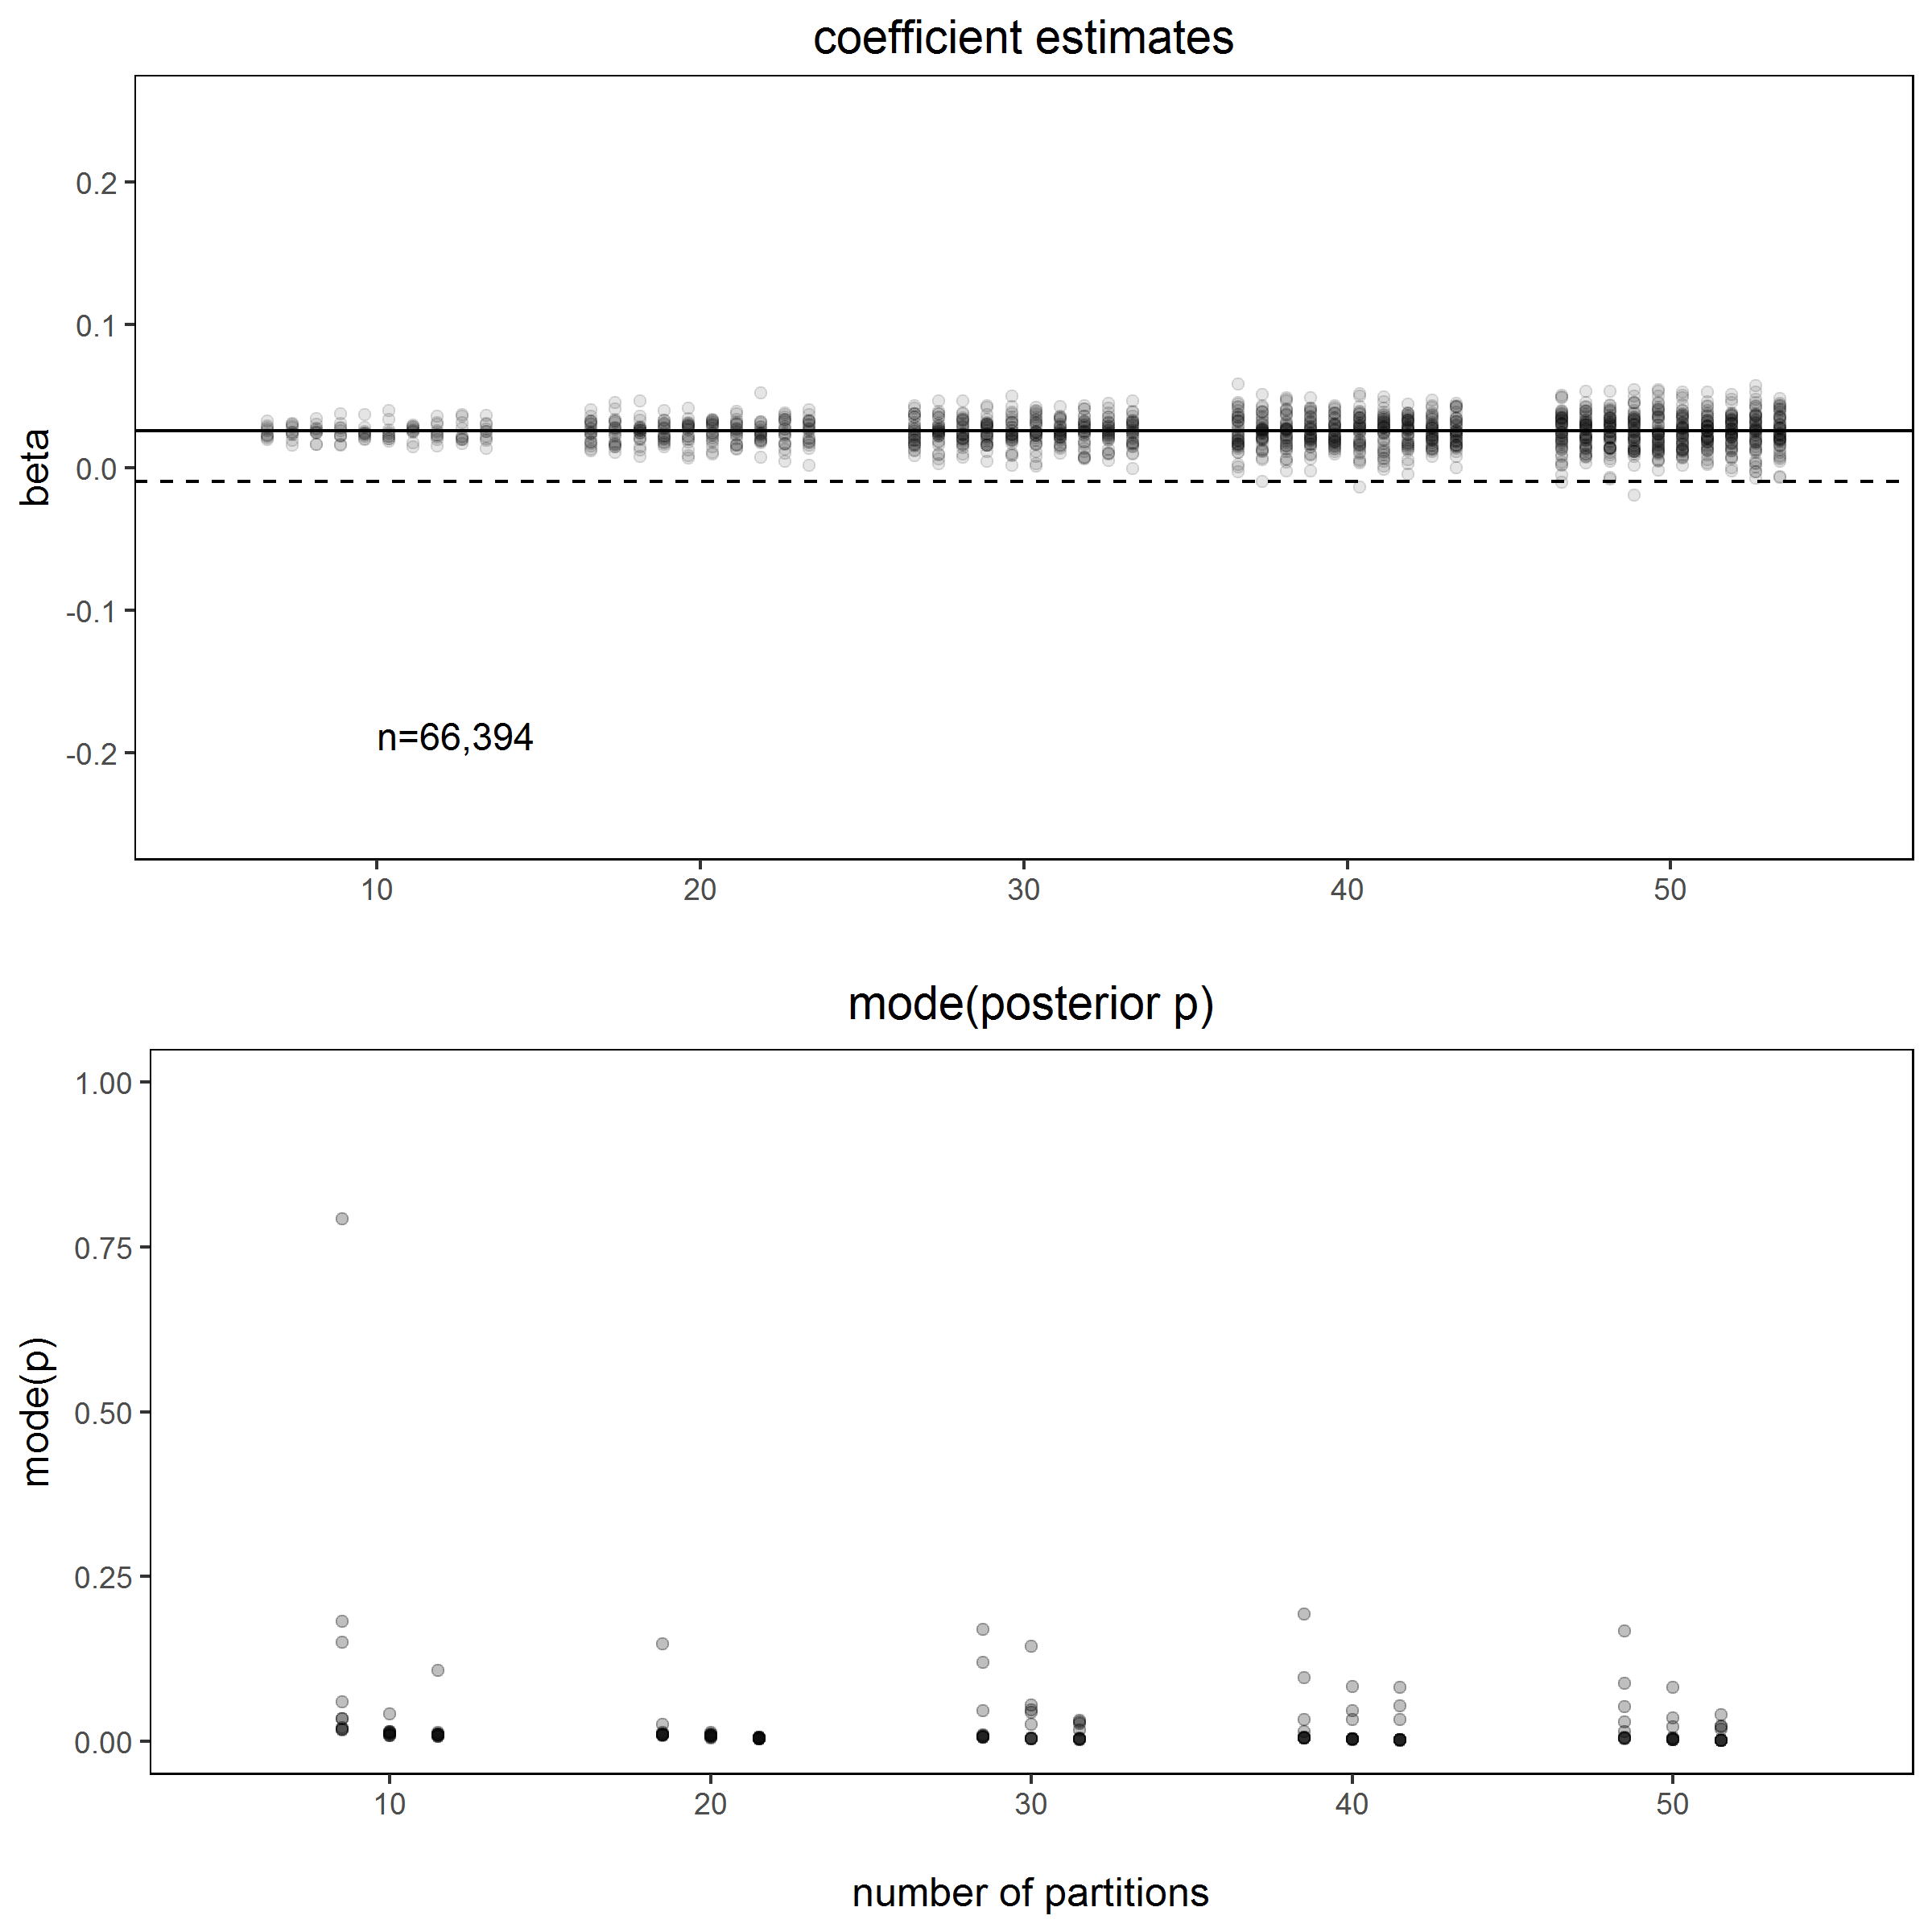
\includegraphics[width=5in]{images/RacePayDifferentialBetaWithPosteriorDistribution-VATA-620-F-C.png}
    \caption{Parameter estimate distribution with distribution of posterior p modes for model (\ref{model:OPM-lnPay-Race}), \textbf{VATA-620-F-C, Veterans Admin, Practical Nurse, Female, Black}.  Ten iterations of random pseudo ID partition generation.  Number of partitions on x-axis.  Dashed line is threshold.  Solid line, given as reference, is disparity coefficient estimate from entire synthetic data set.  Posterior p distributions generated using $\epsilon$ = 0.5, 1.0, and 2.0.}
    \label{figure:RacePayDifferentialBetaWithPosteriorDistribution-VATA-620-F-C}
\end{figure}

\clearpage

\begin{figure}[h!]
    \centering
    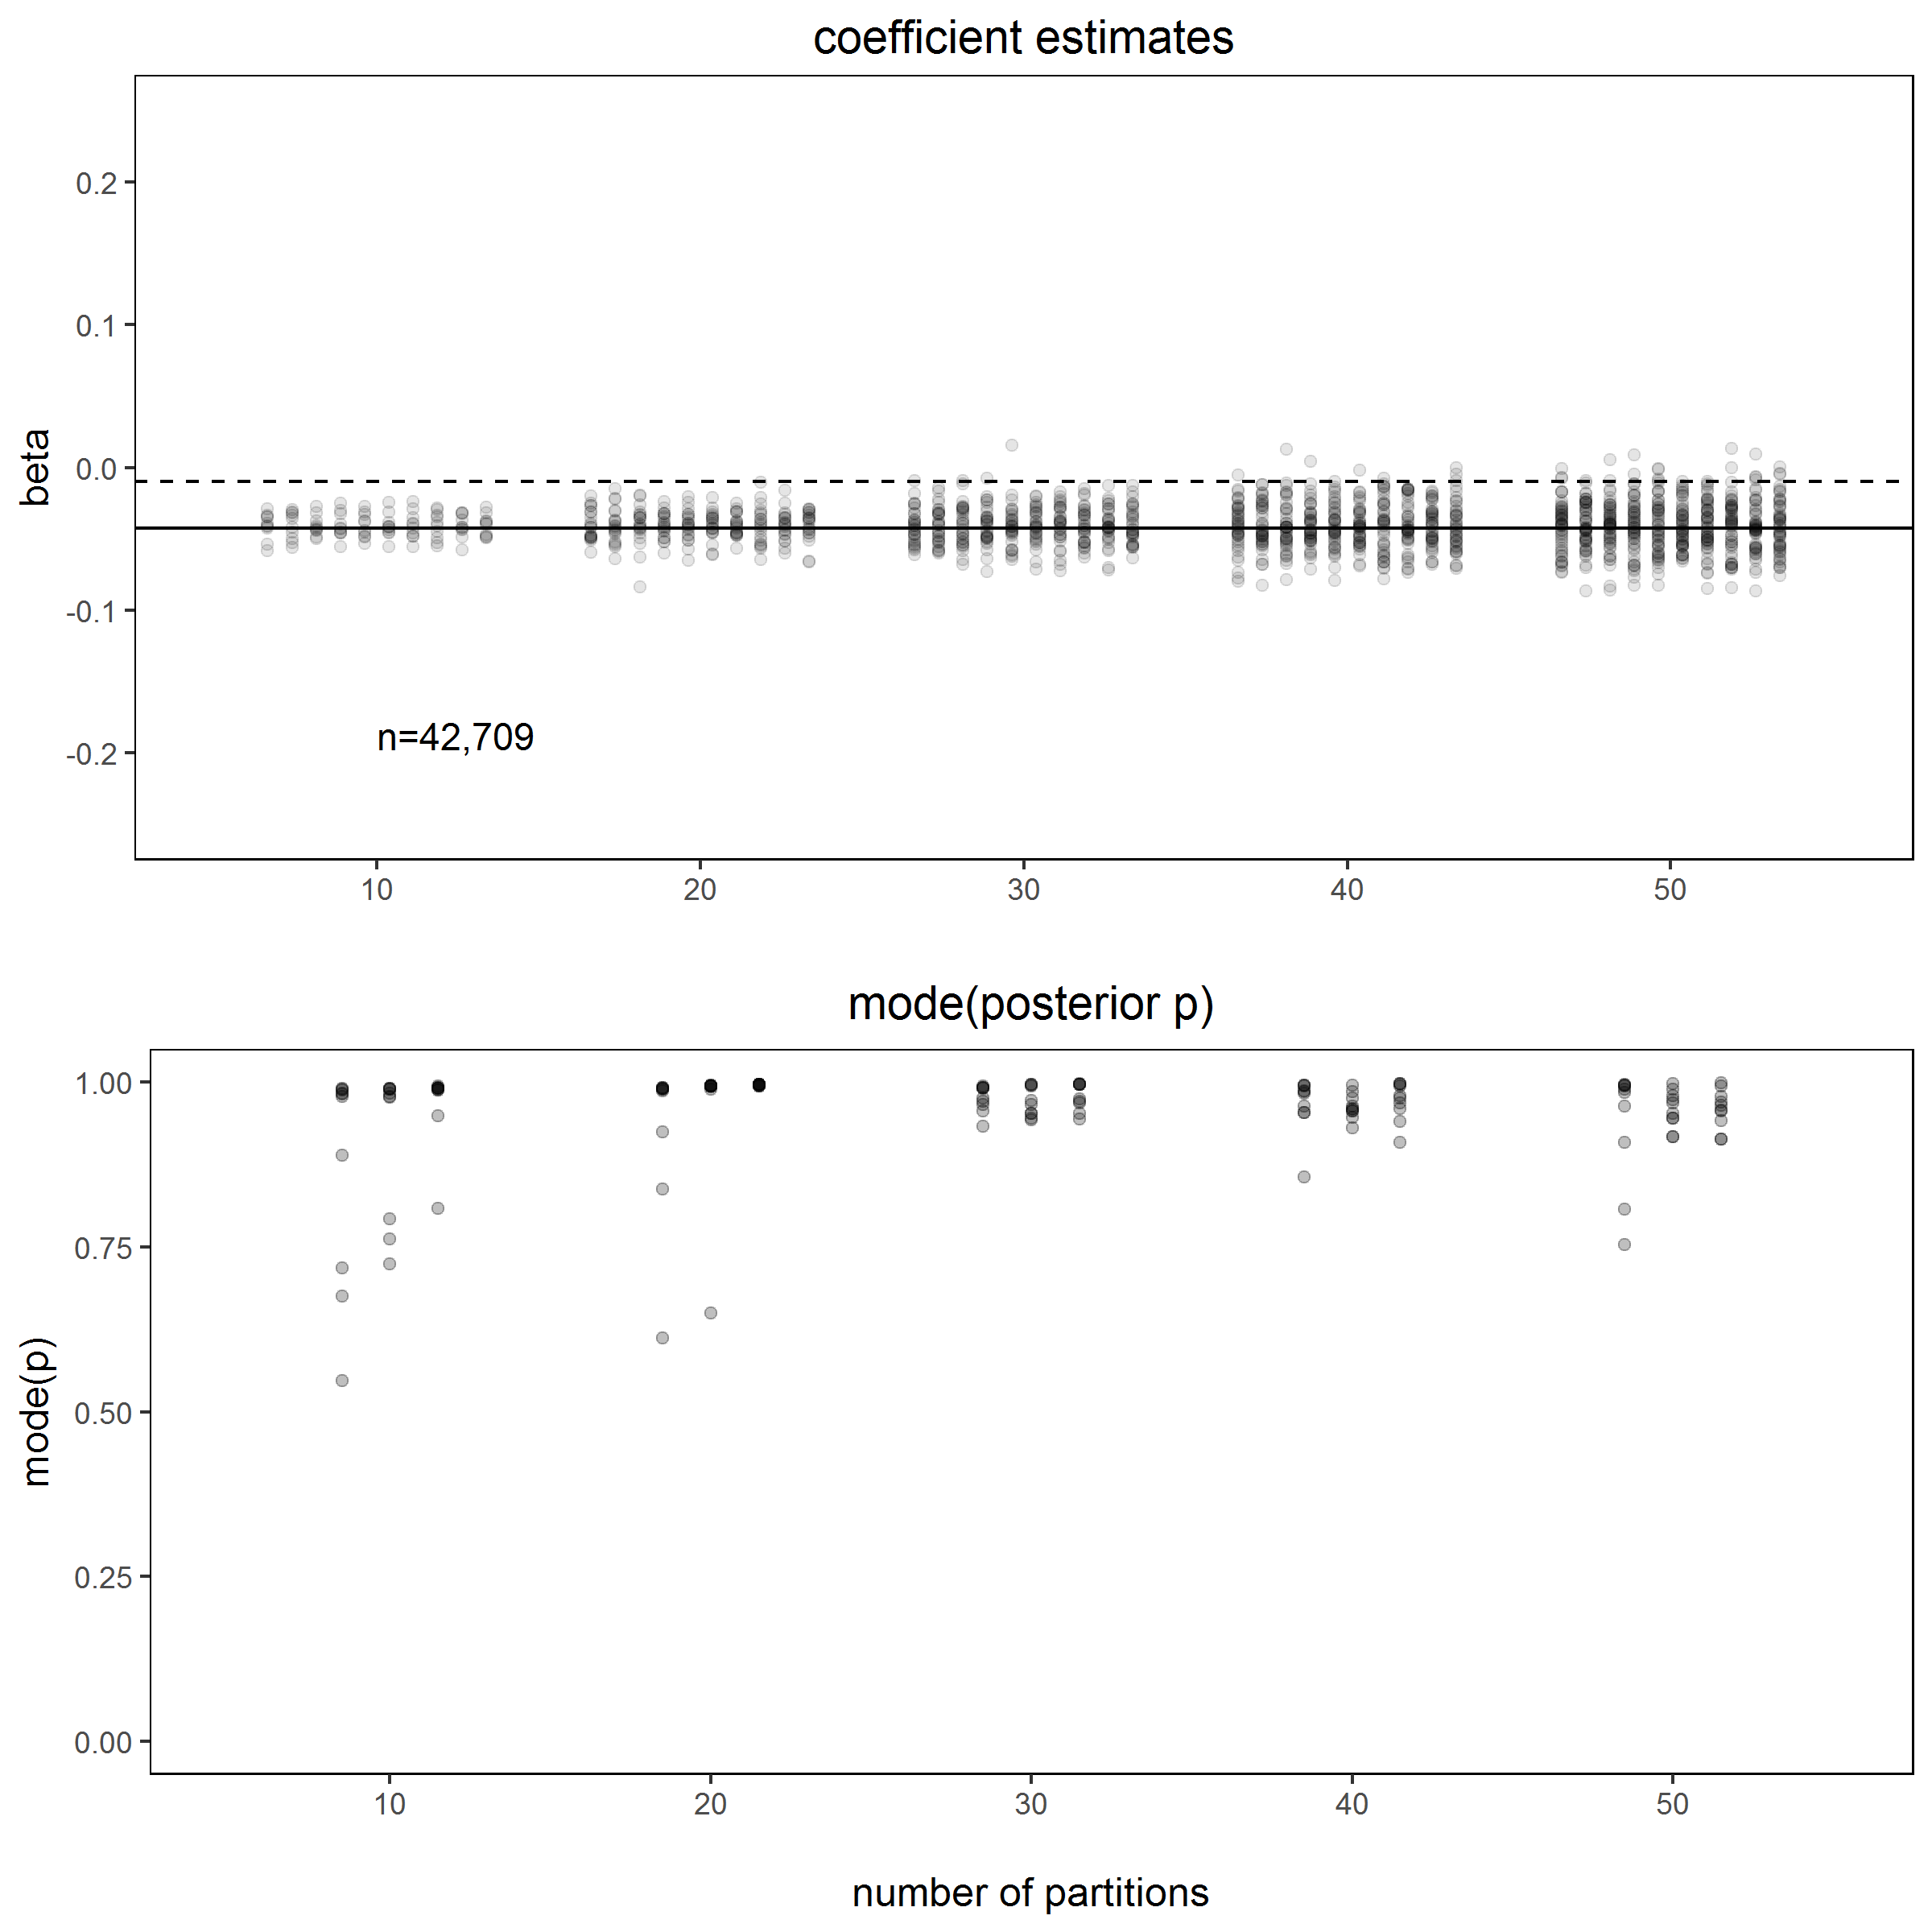
\includegraphics[width=5in]{images/RacePayDifferentialBetaWithPosteriorDistribution-SZ00-105-F-D.png}
    \caption{Parameter estimate distribution with distribution of posterior p modes for model (\ref{model:OPM-lnPay-Race}), \textbf{SZ00-105-F-D, Social Security Admin, Social Insurance Administrator, Female, Hispanic}.  Ten iterations of random pseudo ID partition generation.  Number of partitions on x-axis.  Dashed line is threshold.  Solid line, given as reference, is disparity coefficient estimate from entire synthetic data set.  Posterior p distributions generated using $\epsilon$ = 0.5, 1.0, and 2.0.}
    \label{figure:RacePayDifferentialBetaWithPosteriorDistribution-SZ00-105-F-D}
\end{figure}

\clearpage

\begin{figure}[h!]
    \centering
    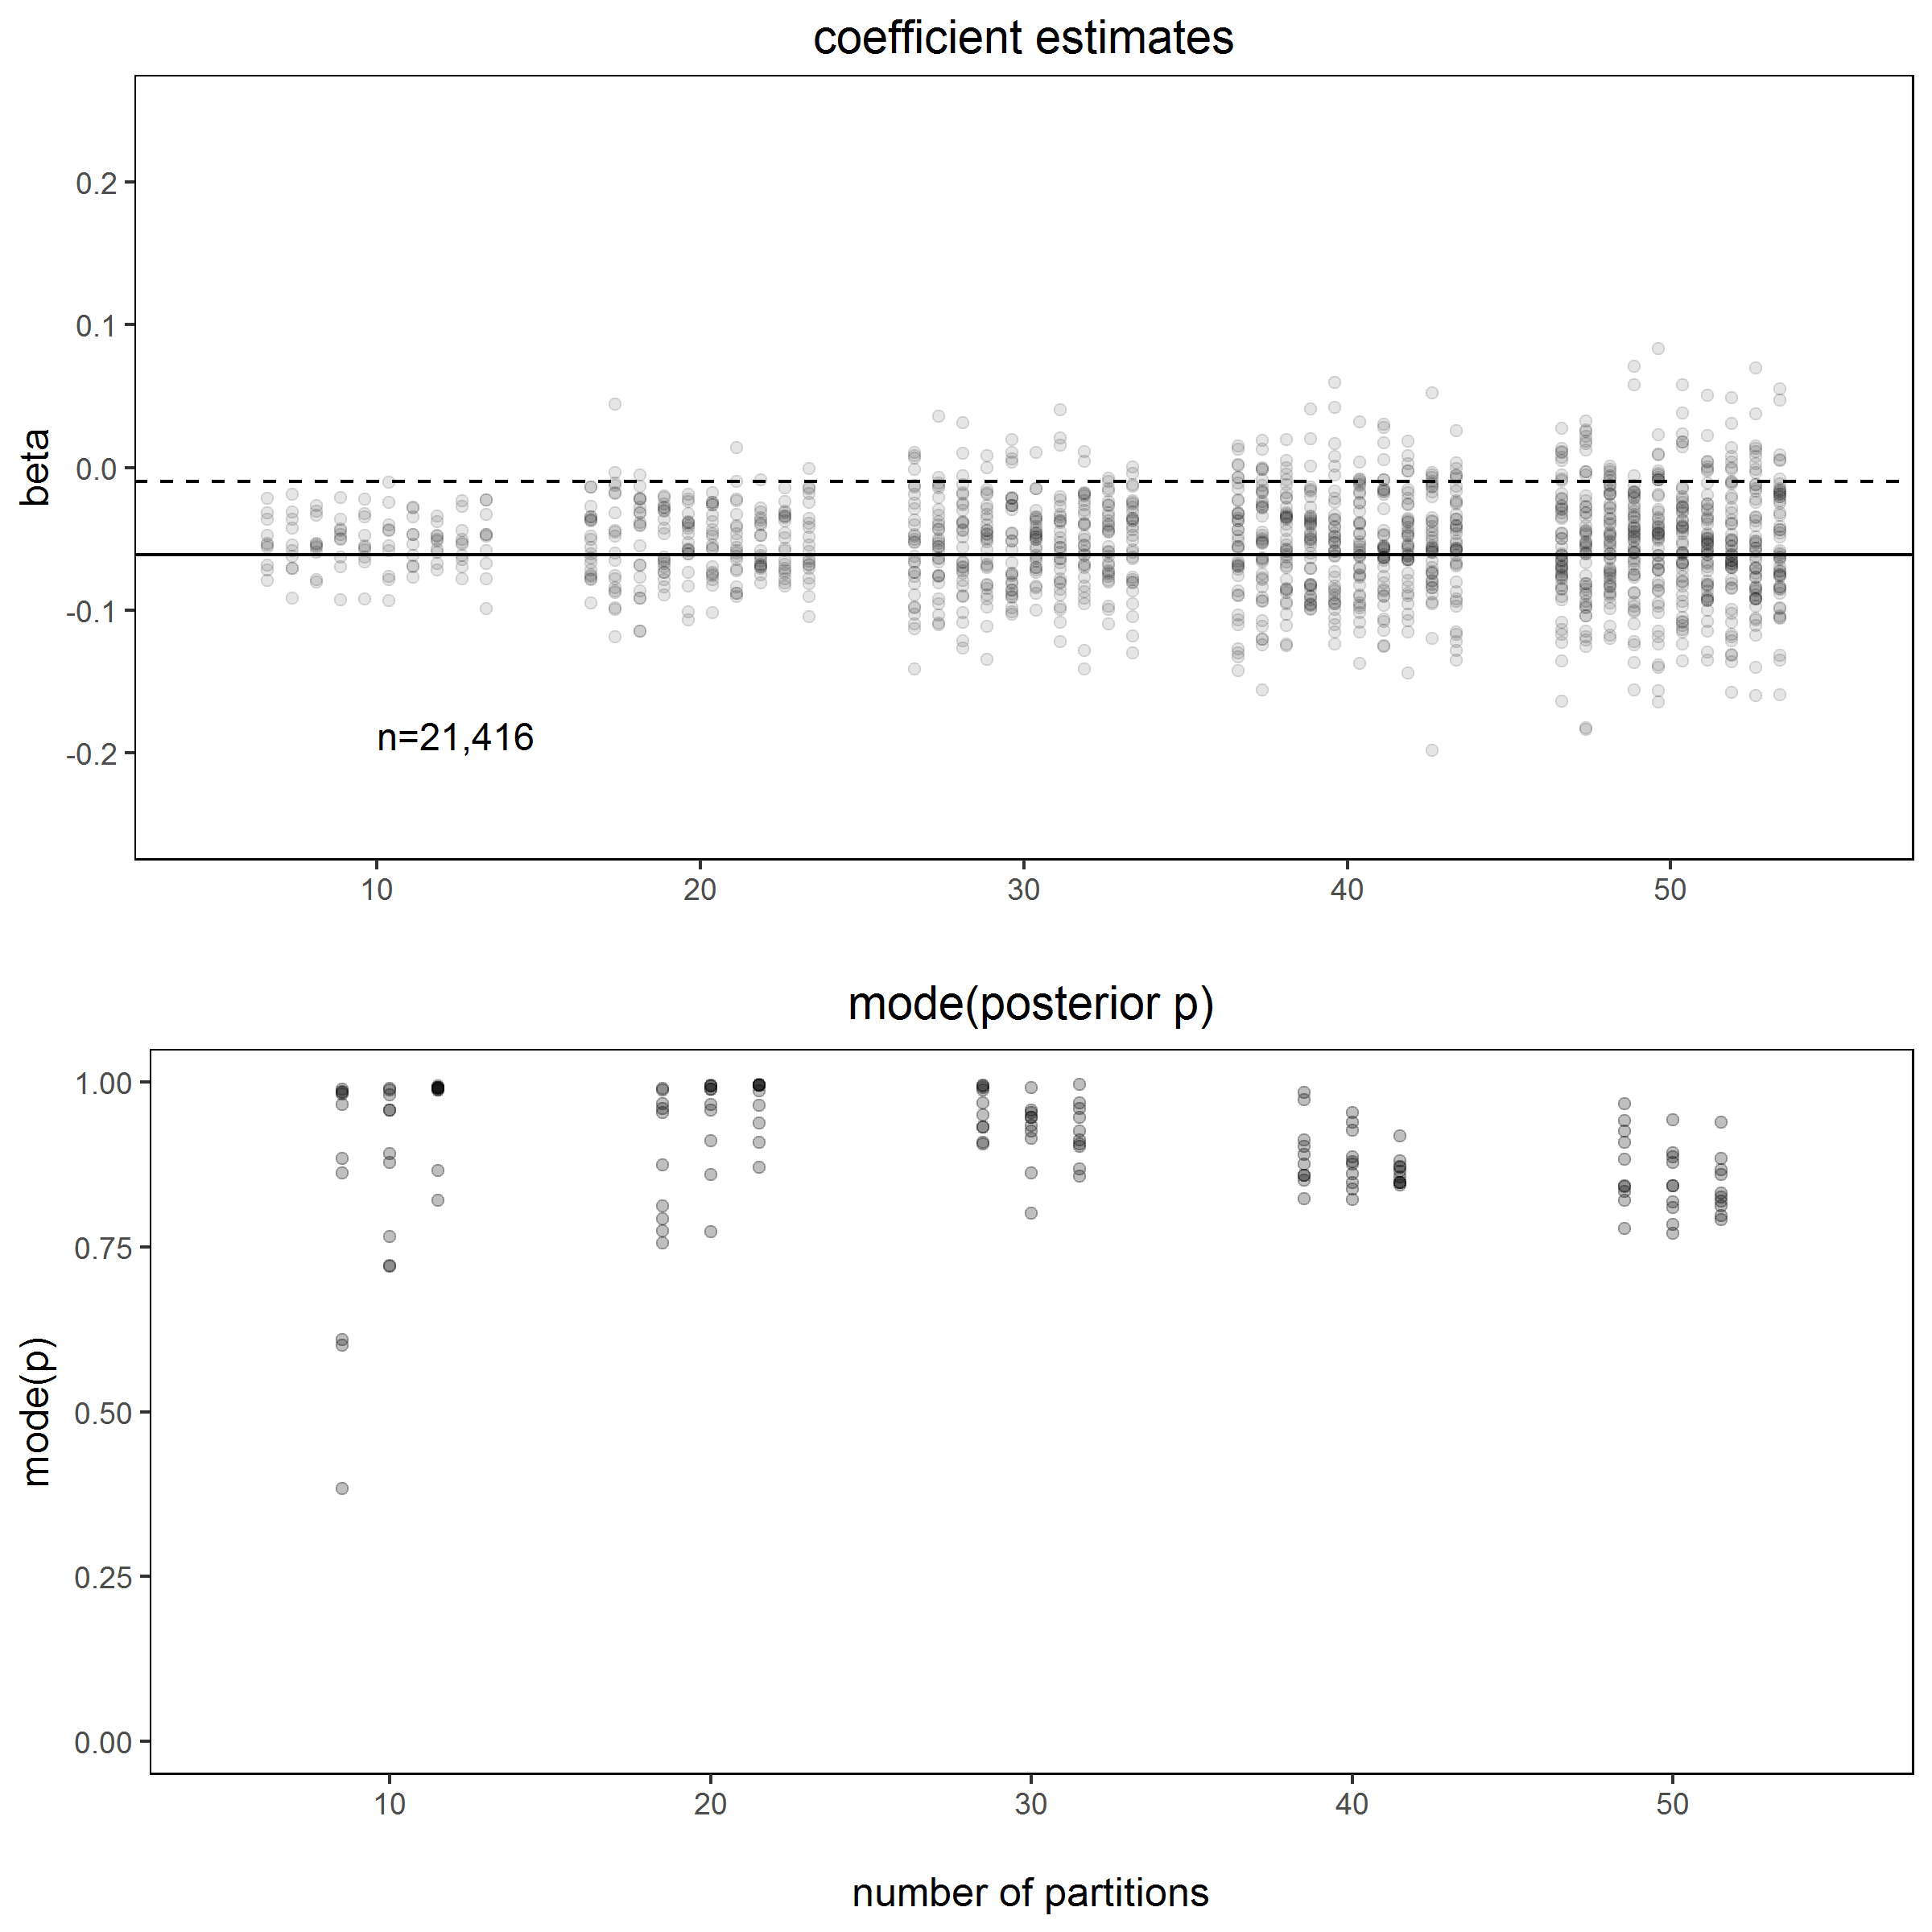
\includegraphics[width=5in]{images/RacePayDifferentialBetaWithPosteriorDistribution-TD03-2152-M-C.png}
    \caption{Parameter estimate distribution with distribution of posterior p modes for model (\ref{model:OPM-lnPay-Race}), \textbf{TD03-2152-M-C, FAA, Air Traffic Controller, Male, Black}.  Ten iterations of random pseudo ID partition generation.  Number of partitions on x-axis.  Dashed line is threshold.  Solid line, given as reference, is disparity coefficient estimate from entire synthetic data set.  Posterior p distributions generated using $\epsilon$ = 0.5, 1.0, and 2.0.}
    \label{figure:RacePayDifferentialBetaWithPosteriorDistribution-TD03-2152-M-C}
\end{figure}

\clearpage

\begin{figure}[h!]
    \centering
    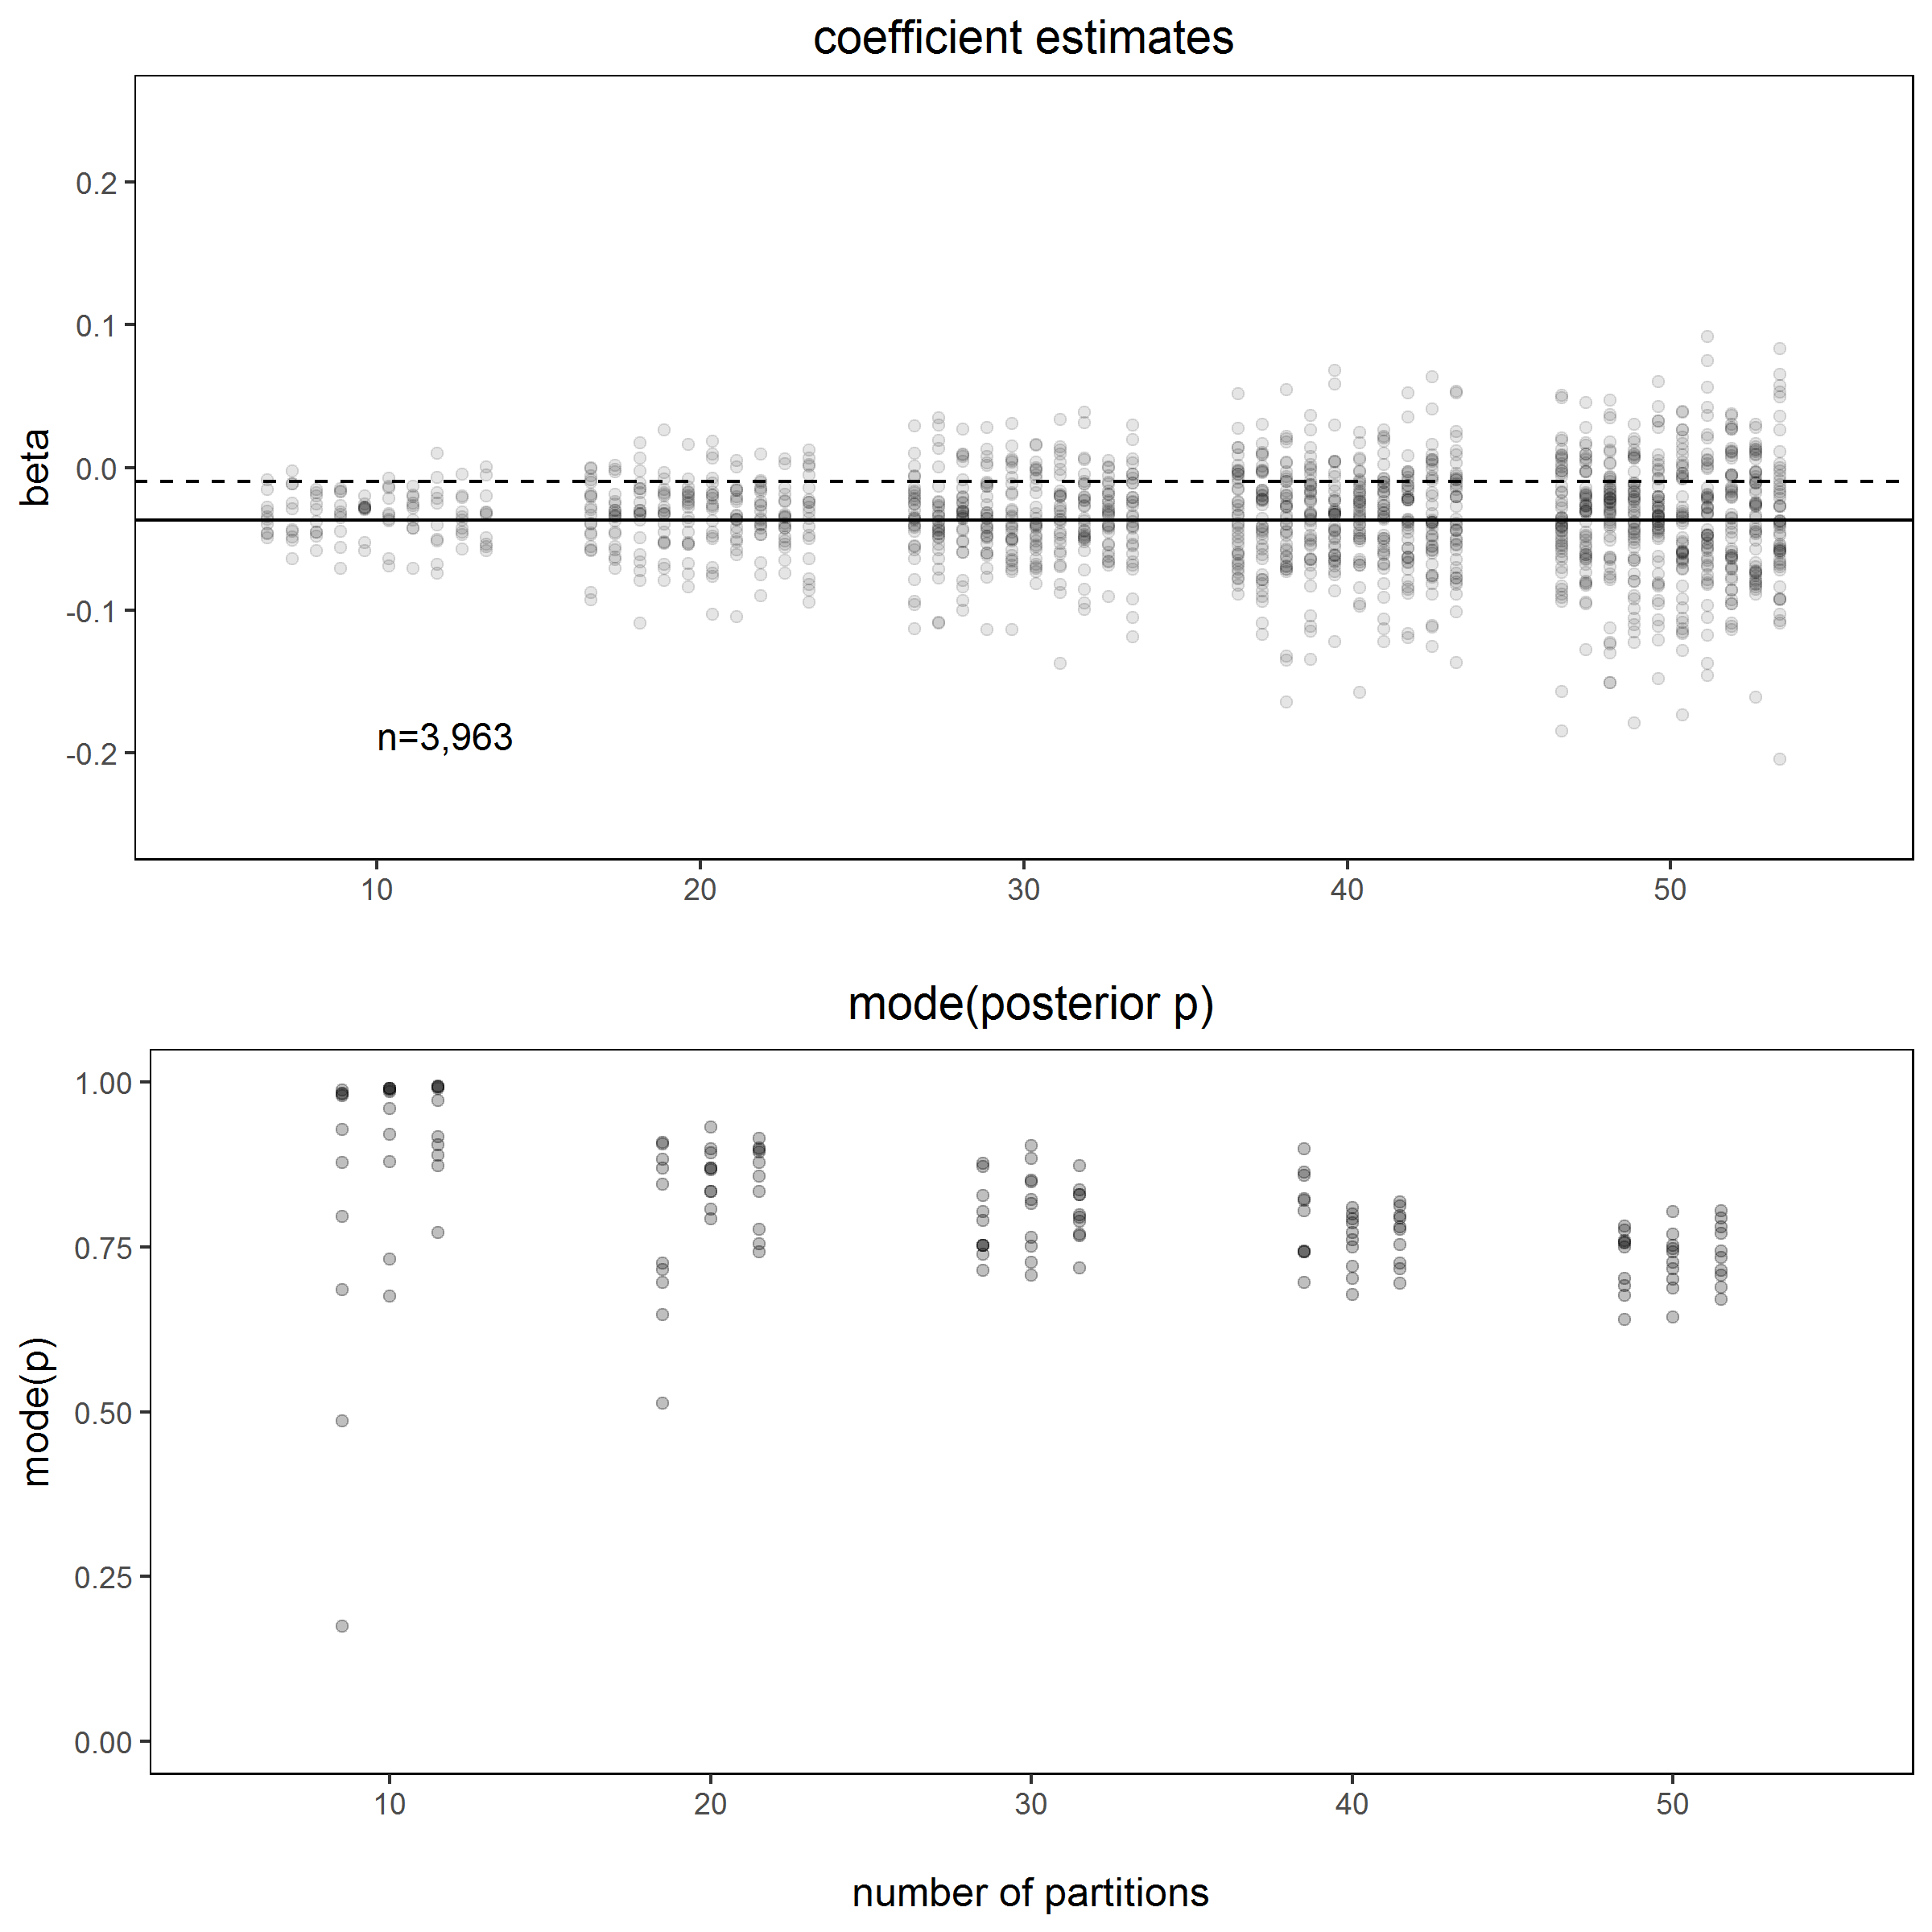
\includegraphics[width=5in]{images/RacePayDifferentialBetaWithPosteriorDistribution-TR93-592-F-B.png}
    \caption{Parameter estimate distribution with distribution of posterior p modes for model (\ref{model:OPM-lnPay-Race}), \textbf{TR93-592-F-B, IRS, Tax Examiner, Female, Asian}.  Ten iterations of random pseudo ID partition generation.  Number of partitions on x-axis.  Dashed line is threshold.  Solid line, given as reference, is disparity coefficient estimate from entire synthetic data set.  Posterior p distributions generated using $\epsilon$ = 0.5, 1.0, and 2.0.}
    \label{figure:RacePayDifferentialBetaWithPosteriorDistribution-TR93-592-F-B}
\end{figure}

\clearpage

\begin{figure}[h!]
    \centering
    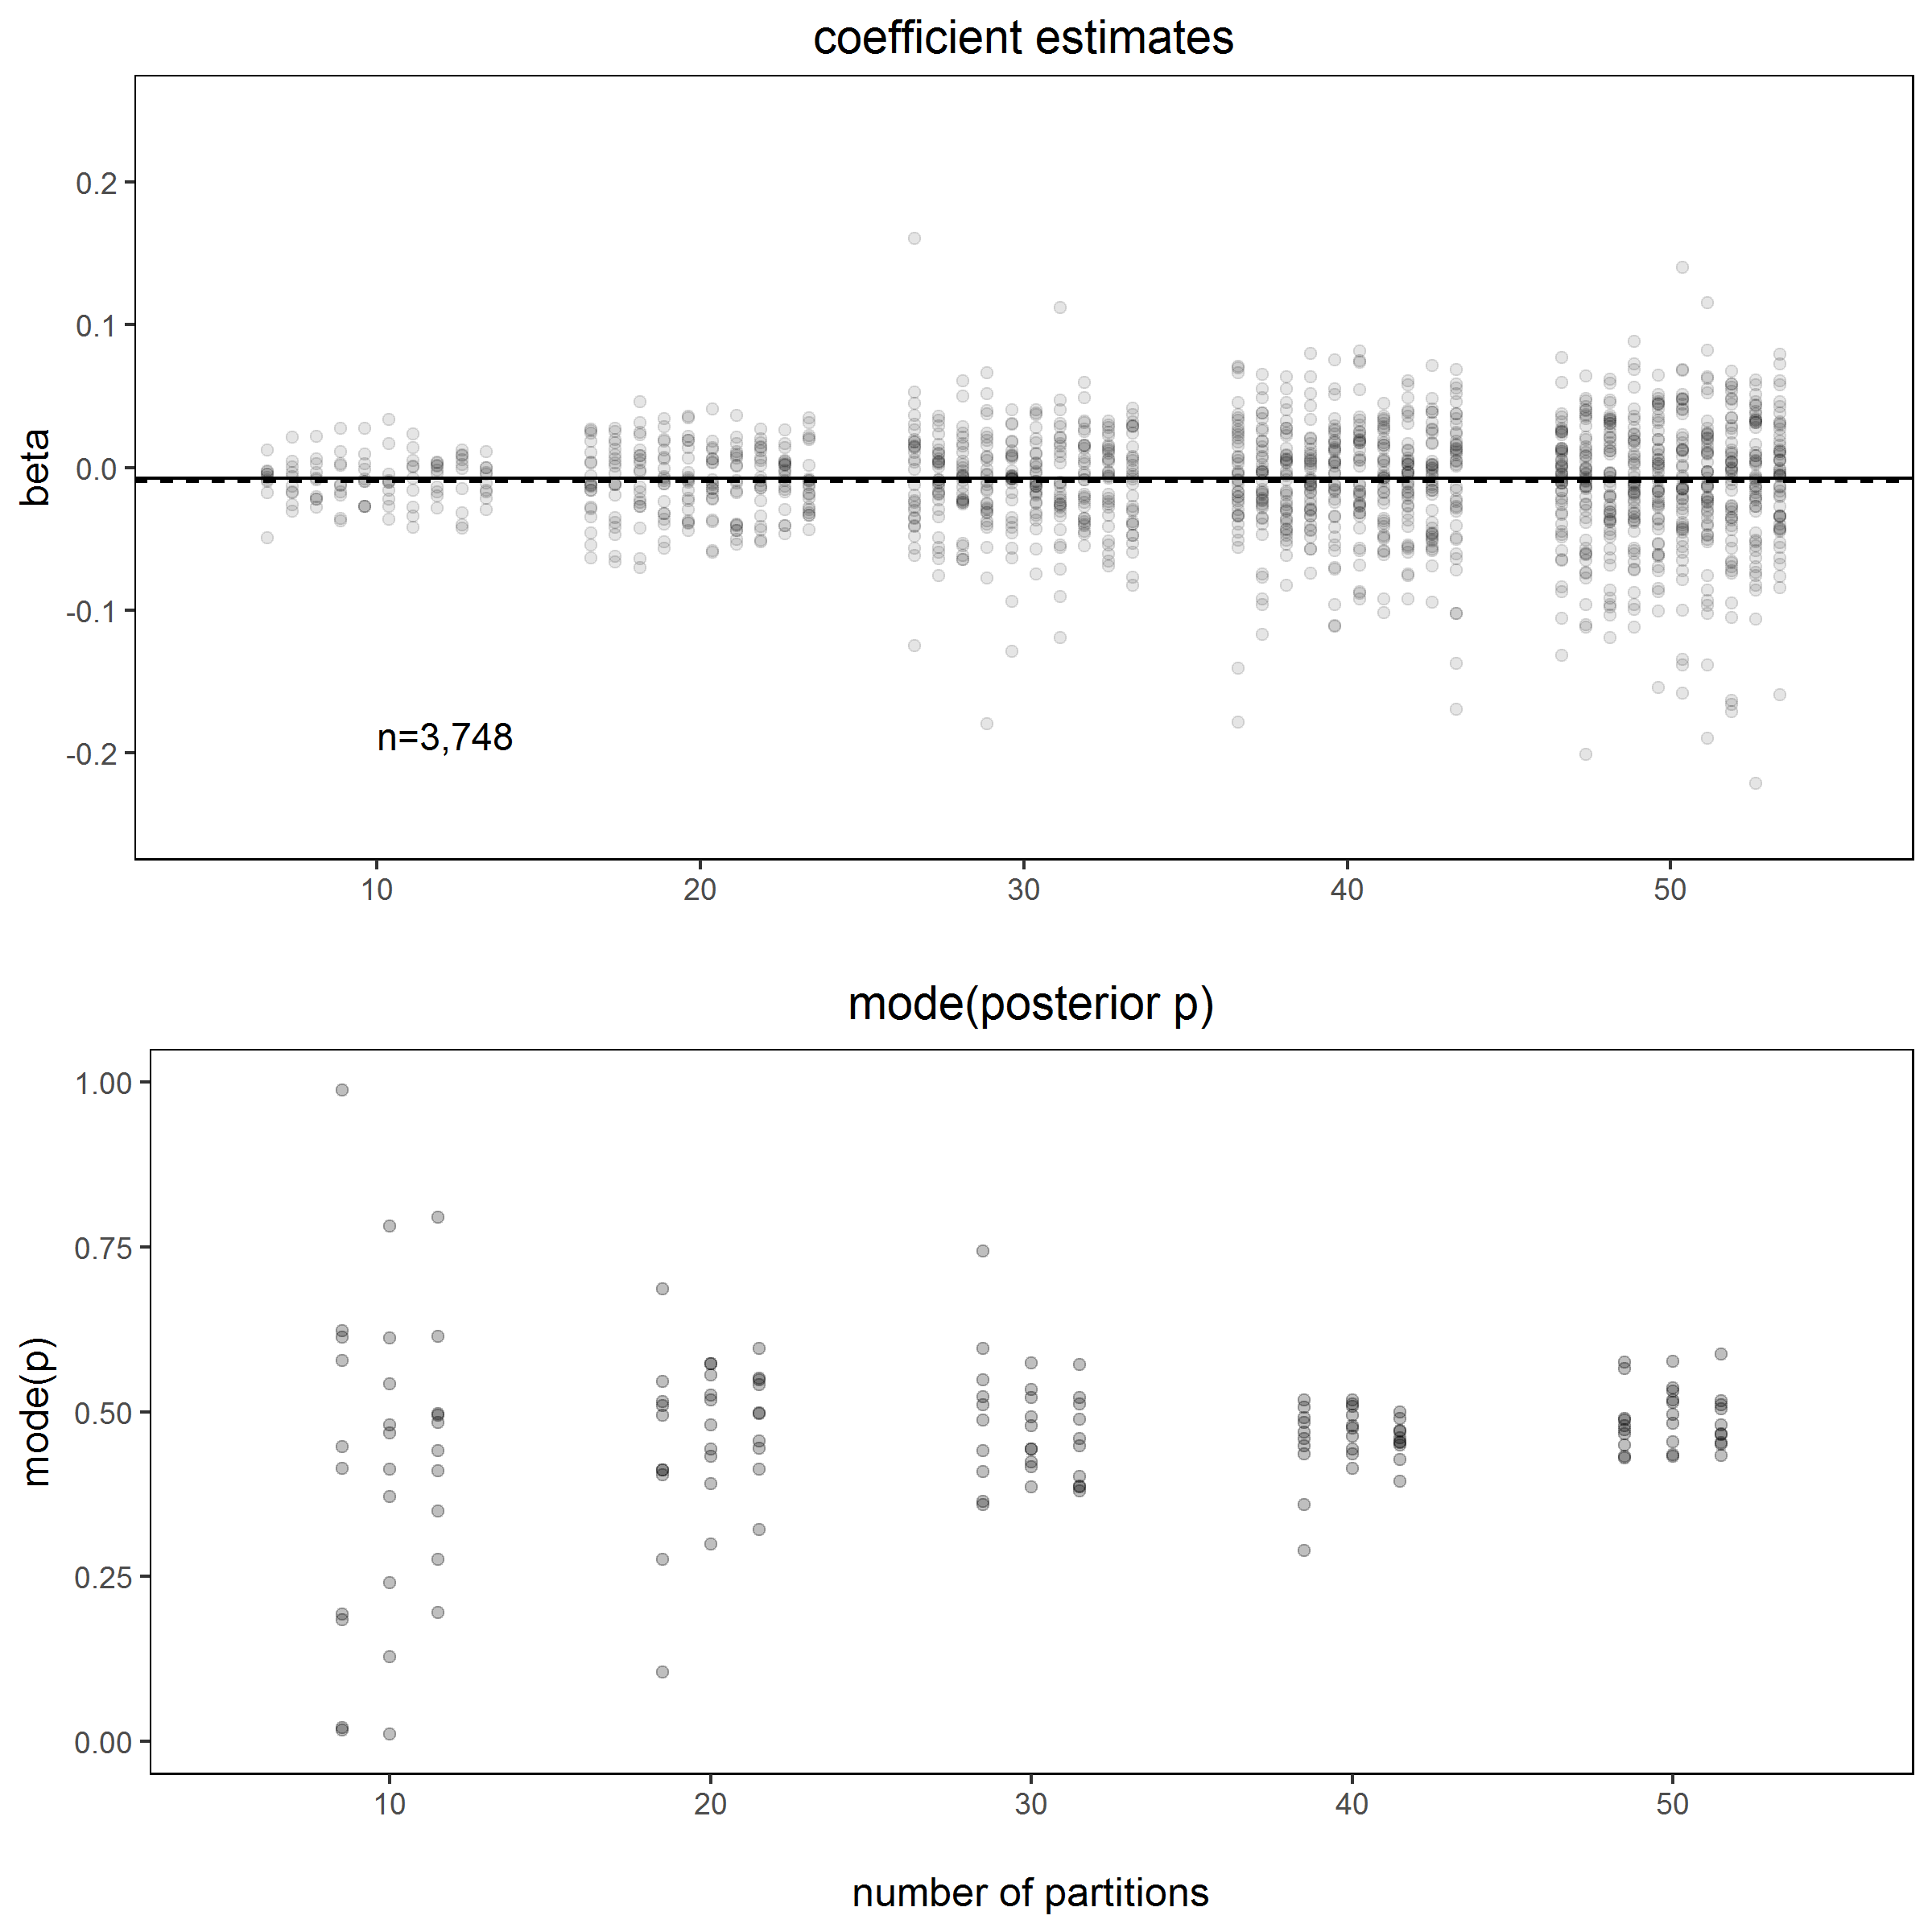
\includegraphics[width=5in]{images/RacePayDifferentialBetaWithPosteriorDistribution-DJ09-905-F-C.png}
    \caption{Parameter estimate distribution with distribution of posterior p modes for model (\ref{model:OPM-lnPay-Race}), \textbf{DJ09-905-F-C, Office of U.S. Attorney, Attorney, Female, Black}.  Ten iterations of random pseudo ID partition generation.  Number of partitions on x-axis.  Dashed line is threshold.  Solid line, given as reference, is disparity coefficient estimate from entire synthetic data set.  Posterior p distributions generated using $\epsilon$ = 0.5, 1.0, and 2.0.}
    \label{figure:RacePayDifferentialBetaWithPosteriorDistribution-DJ09-905-F-C}
\end{figure}

\clearpage

\begin{figure}[h!]
    \centering
    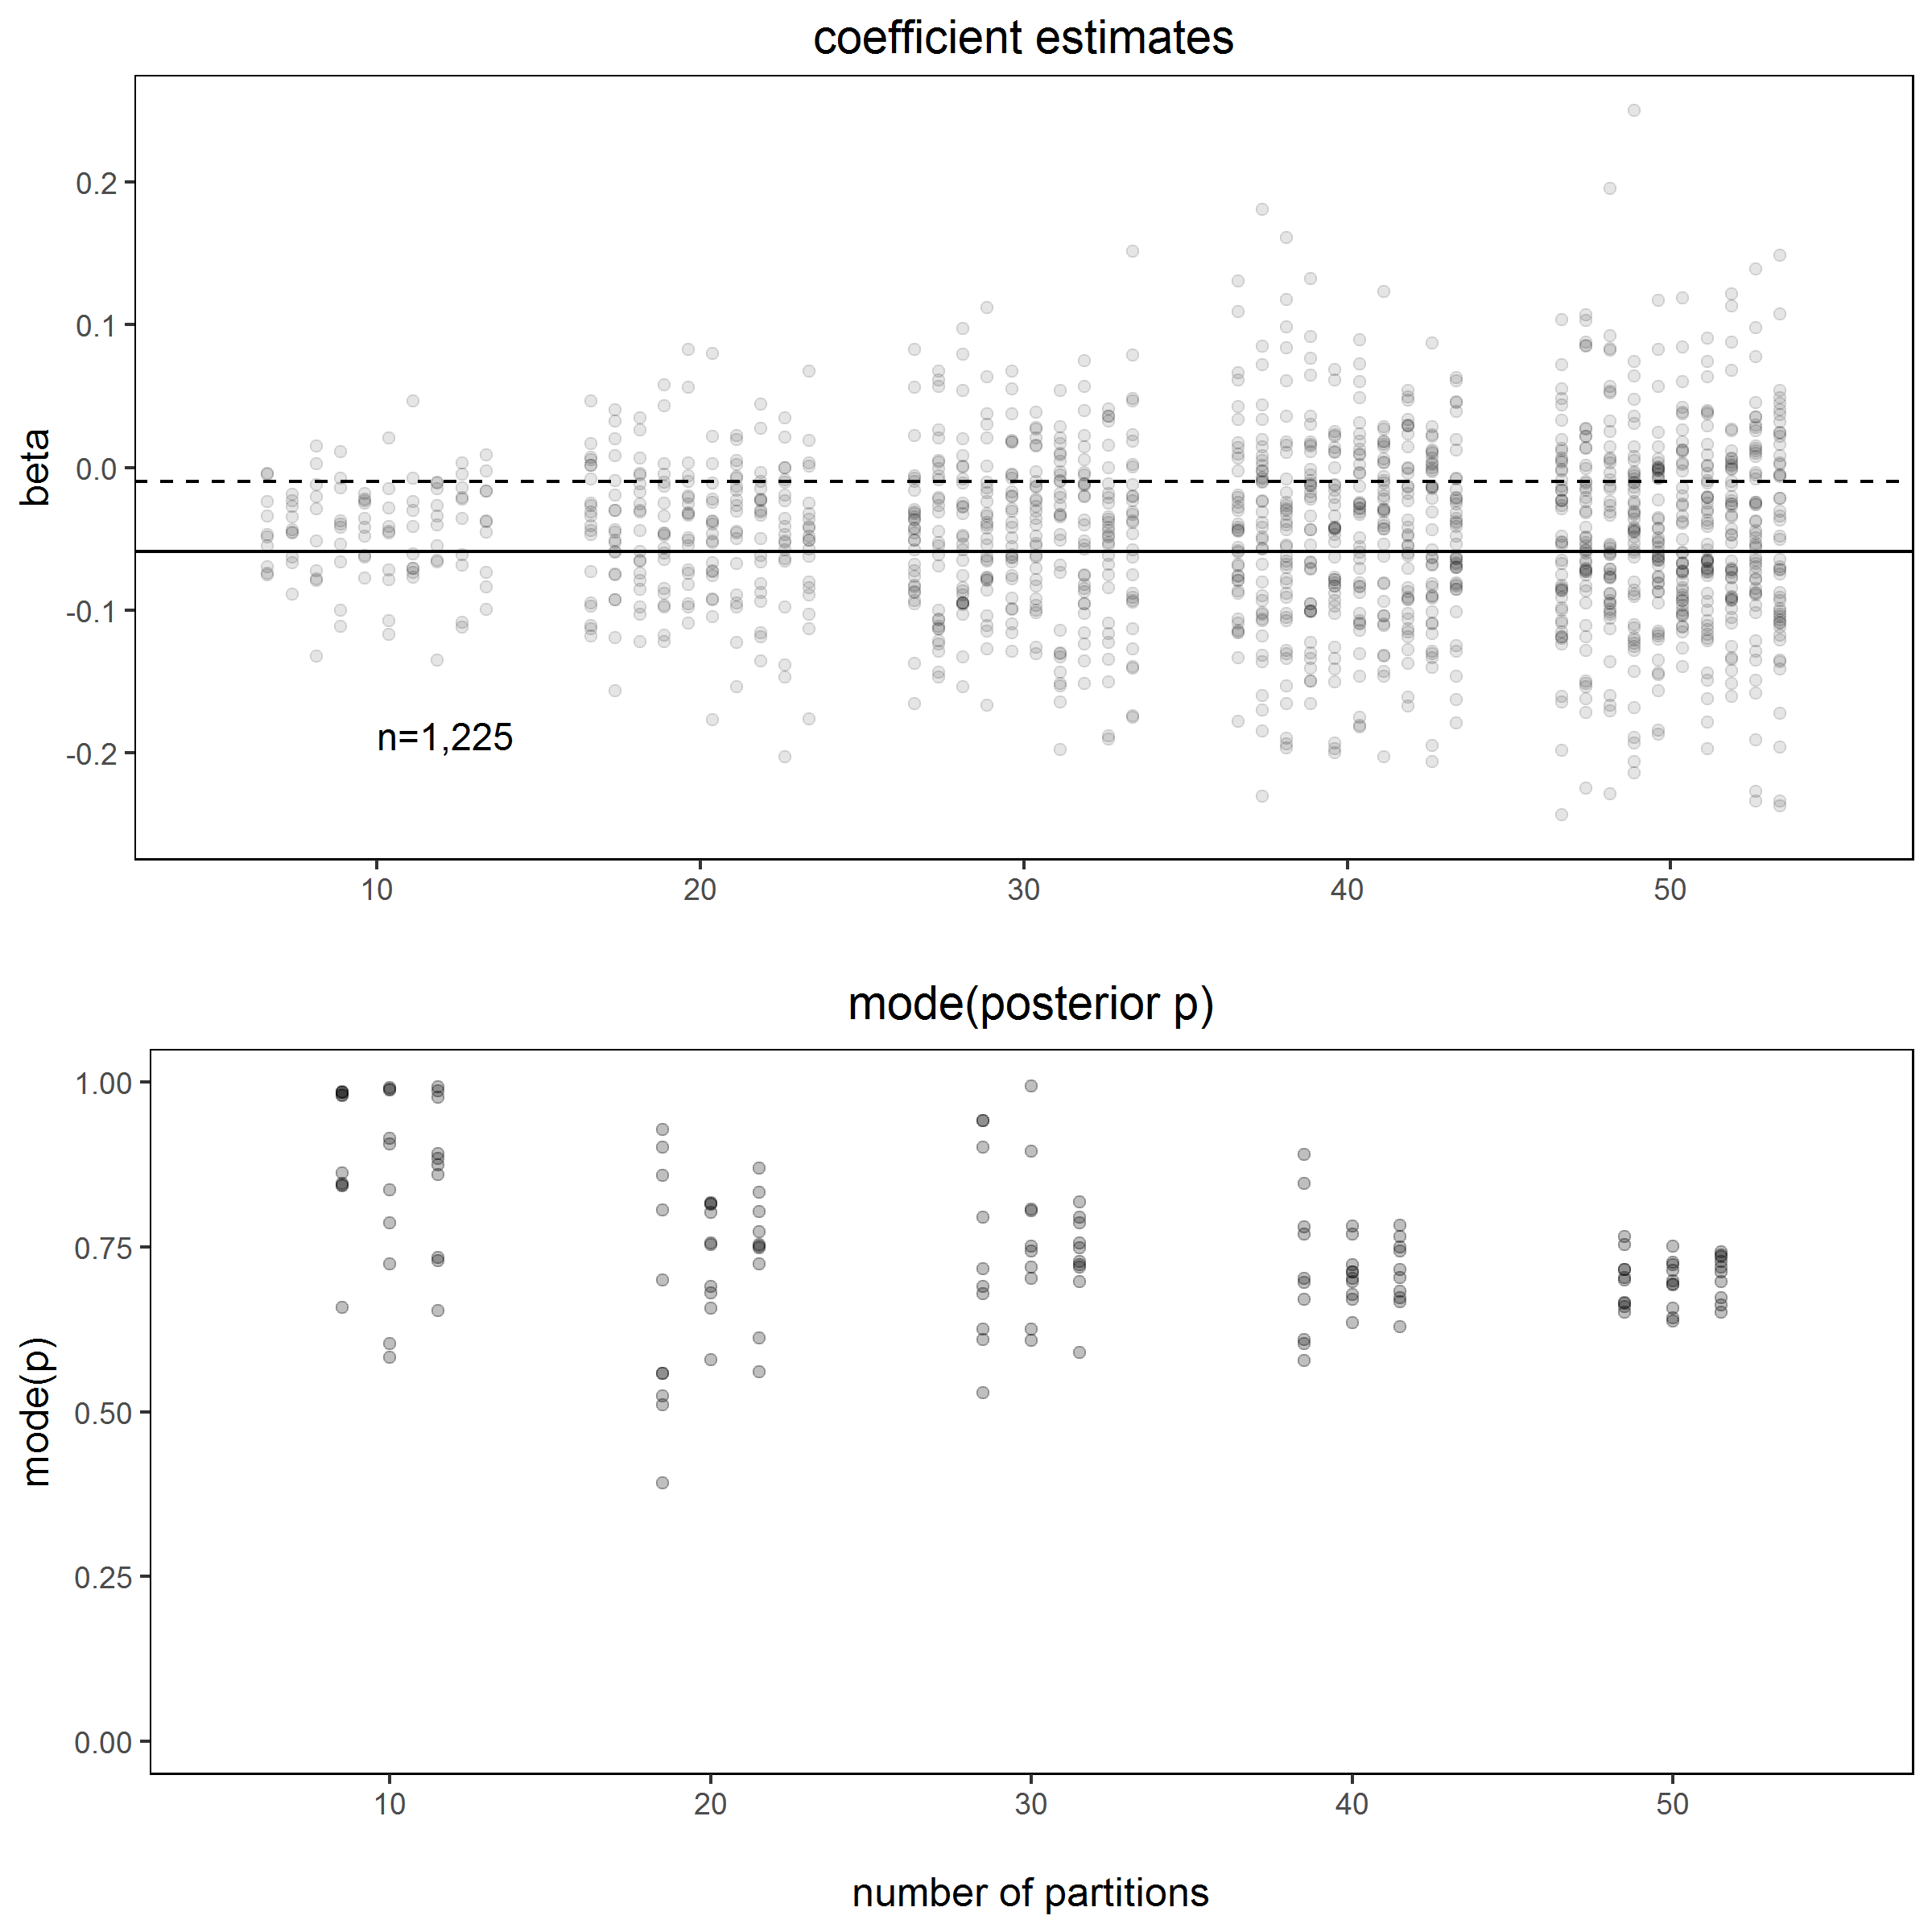
\includegraphics[width=5in]{images/RacePayDifferentialBetaWithPosteriorDistribution-DJ02-1811-F-B.png}
    \caption{Parameter estimate distribution with distribution of posterior p modes for model (\ref{model:OPM-lnPay-Race}), \textbf{DJ02-1811-F-B, FBI, Criminal Investigator, Female, Asian}.  Ten iterations of random pseudo ID partition generation.  Number of partitions on x-axis.  Dashed line is threshold.  Solid line, given as reference, is disparity coefficient estimate from entire synthetic data set.  Posterior p distributions generated using $\epsilon$ = 0.5, 1.0, and 2.0.}
    \label{figure:RacePayDifferentialBetaWithPosteriorDistribution-DJ02-1811-F-B}
\end{figure}

\clearpage

\begin{figure}[h!]
    \centering
    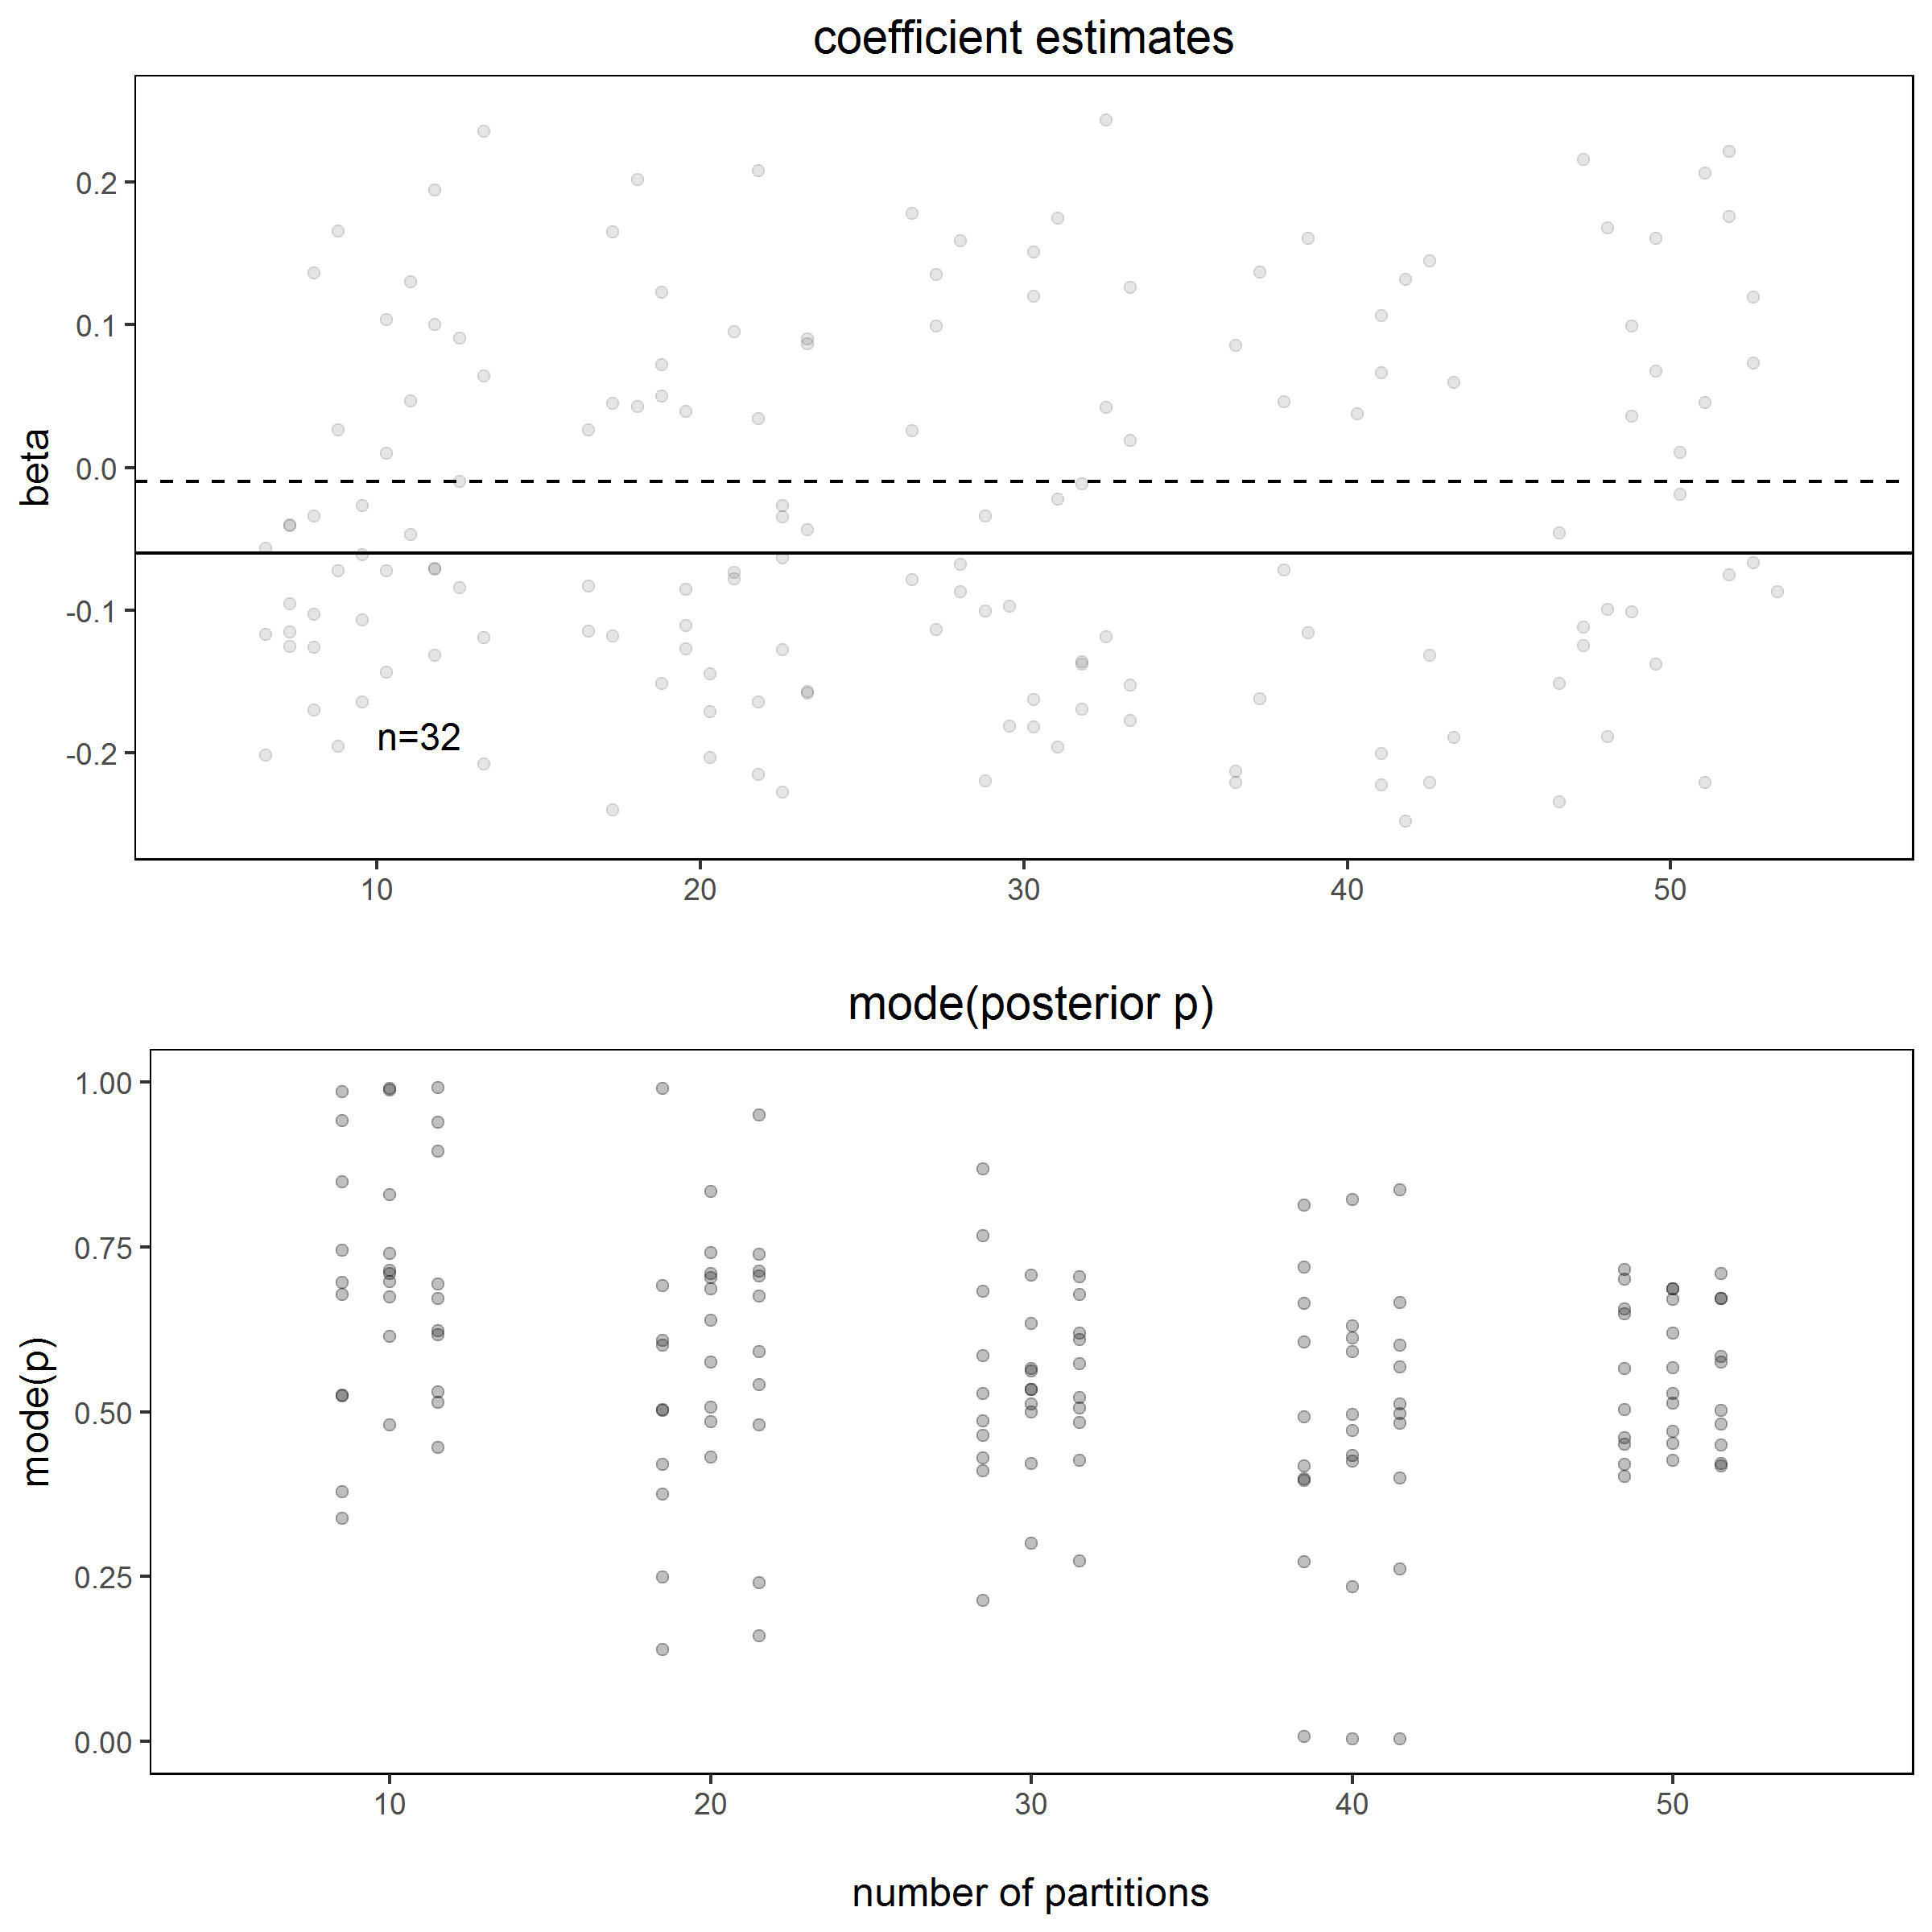
\includegraphics[width=5in]{images/RacePayDifferentialBetaWithPosteriorDistribution-LF00-905-F-B.png}
    \caption{Parameter estimate distribution with distribution of posterior p modes for model (\ref{model:OPM-lnPay-Race}), \textbf{LF00-511-F-B, FEC, Attorney, Female, Black}.  Ten iterations of random pseudo ID partition generation.  Number of partitions on x-axis.  Dashed line is threshold.  Solid line, given as reference, is disparity coefficient estimate from entire synthetic data set.  Posterior p distributions generated using $\epsilon$ = 0.5, 1.0, and 2.0.}
    \label{figure:RacePayDifferentialBetaWithPosteriorDistribution-LF00-905-F-B}
\end{figure}

\clearpage

\begin{figure}[h!]
    \centering
    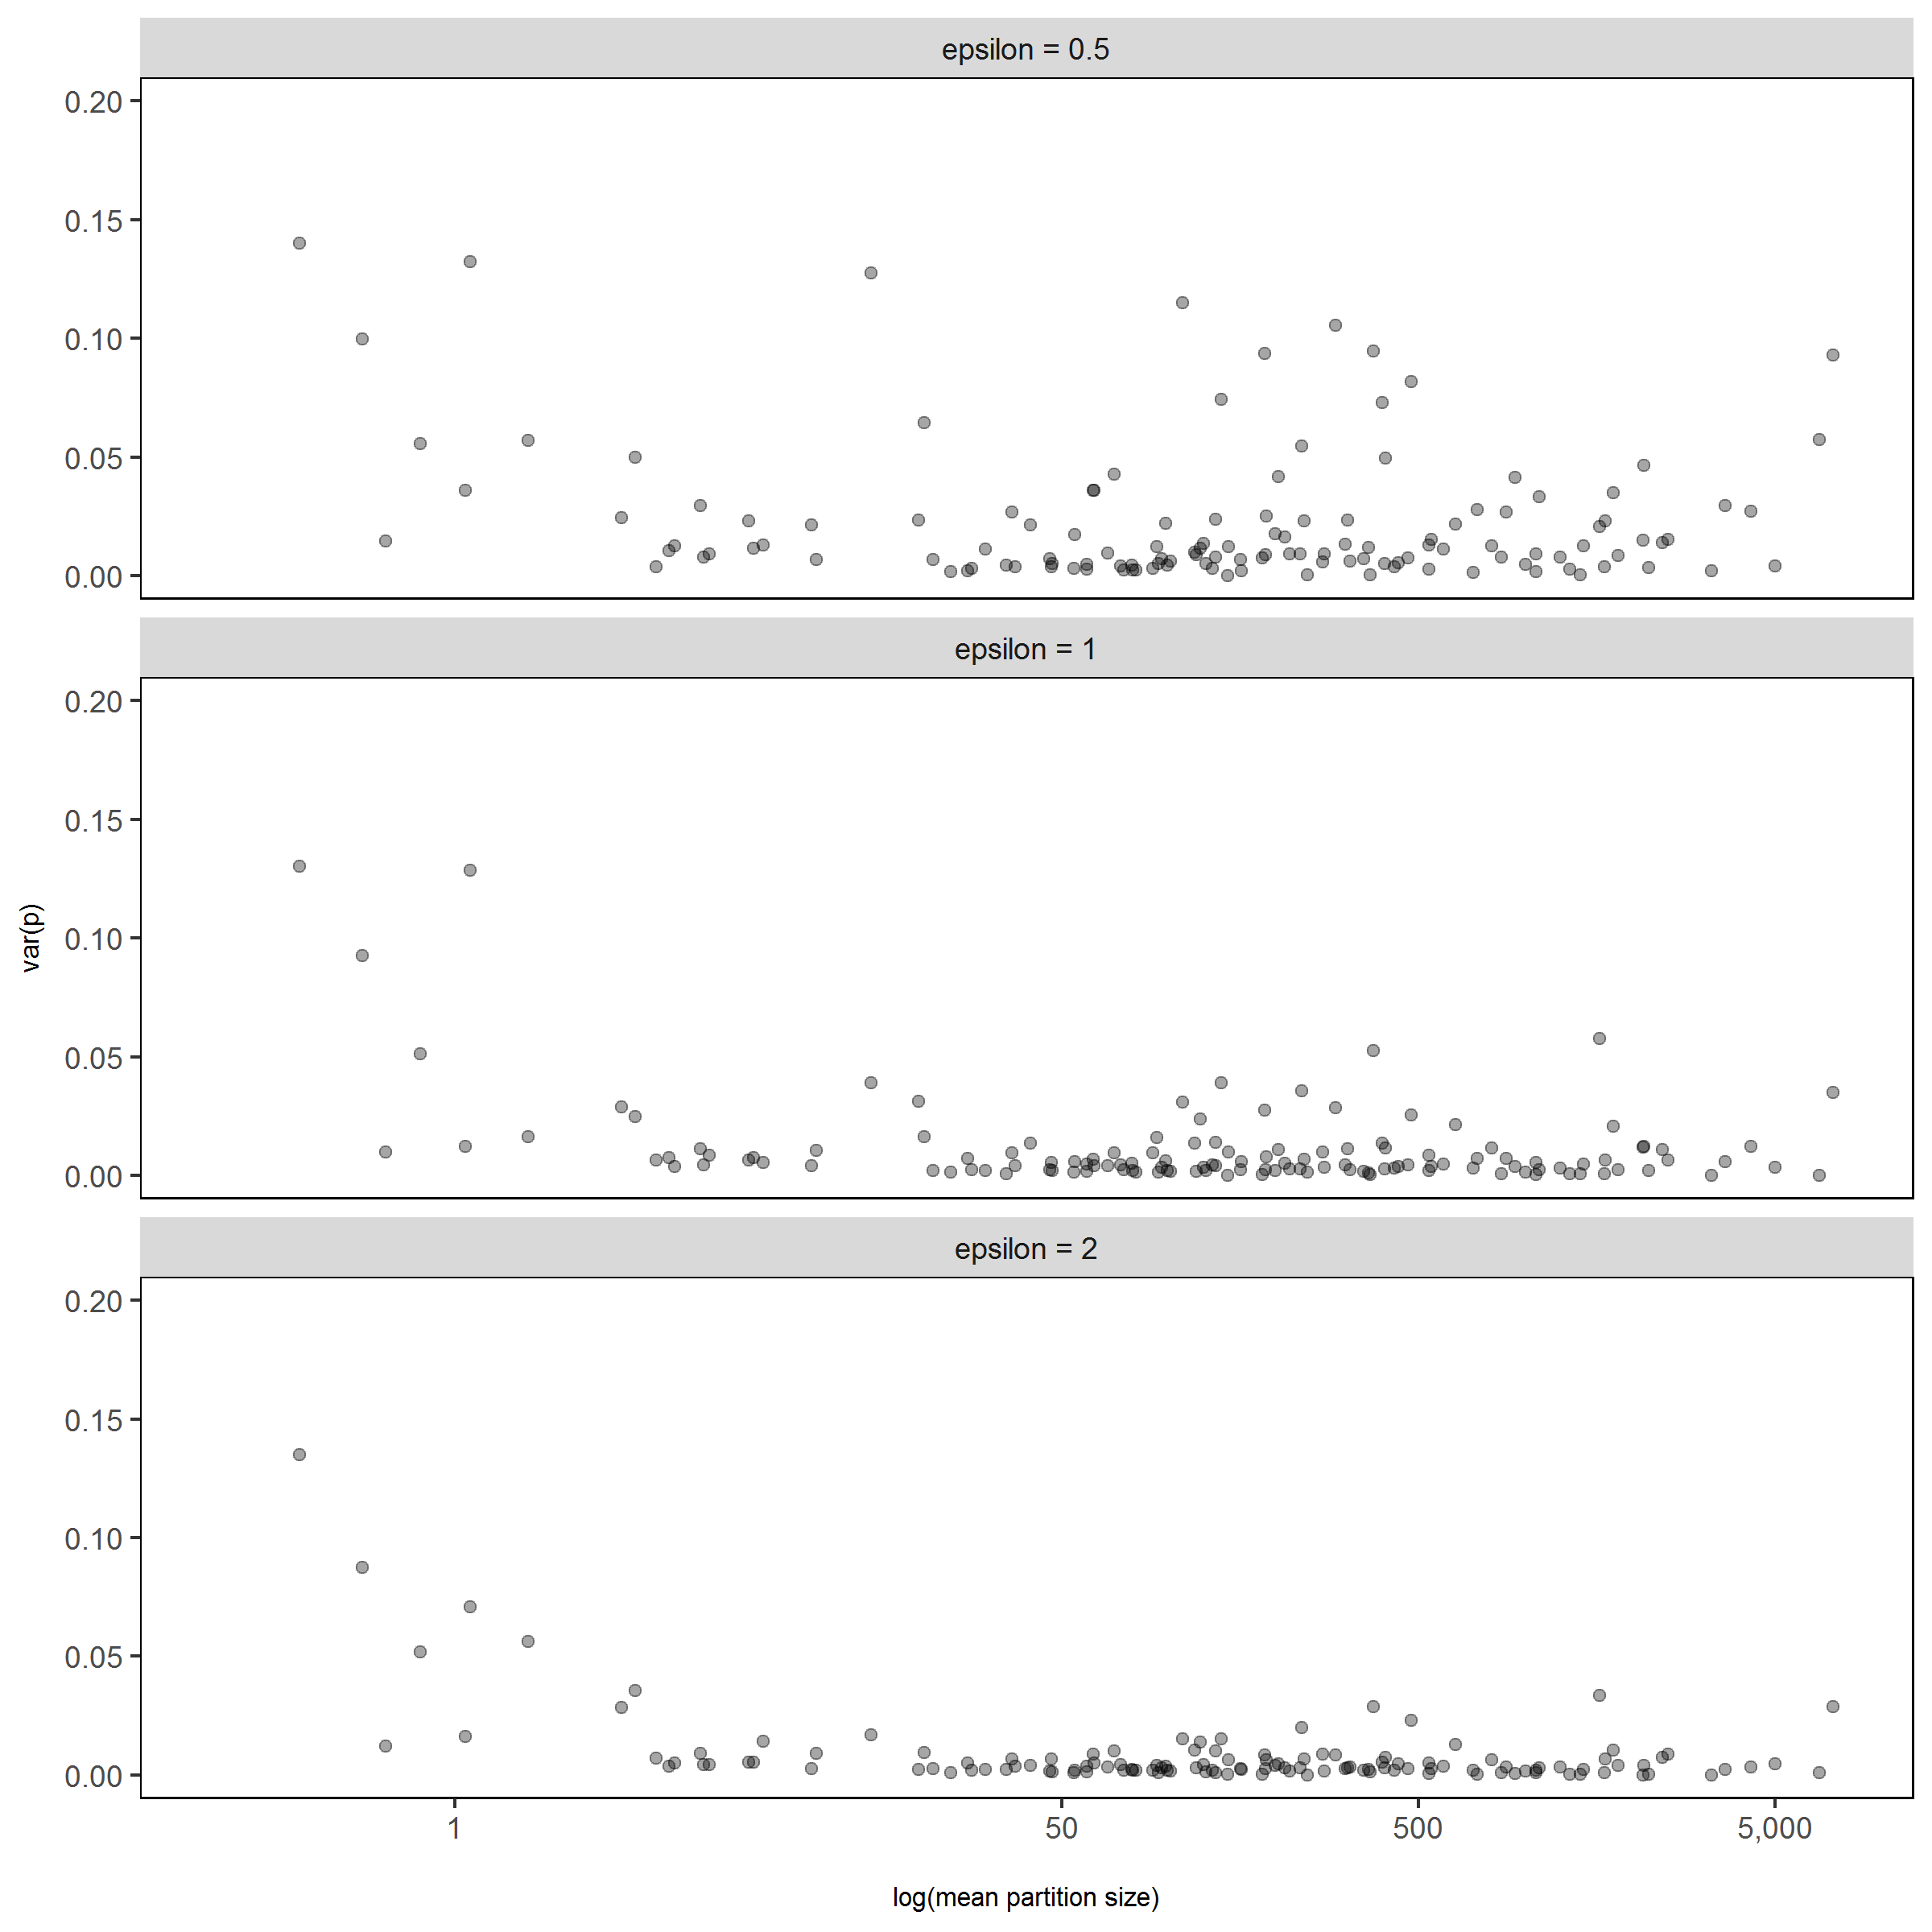
\includegraphics[width=6in]{RacePayDifferential-p-Variance-Partition-Size.png}
    \caption{Variance of posterior p values with respect to partition size.  Each point represents the variance of ten posterior p values, from the ten iterations for each agency, occupation, sex, race, M, and $\epsilon$.}
    \label{figure:RacePayDifferential-p-Variance-Partition-Size}
\end{figure}

\clearpage

\begin{figure}[h!]
    \centering
    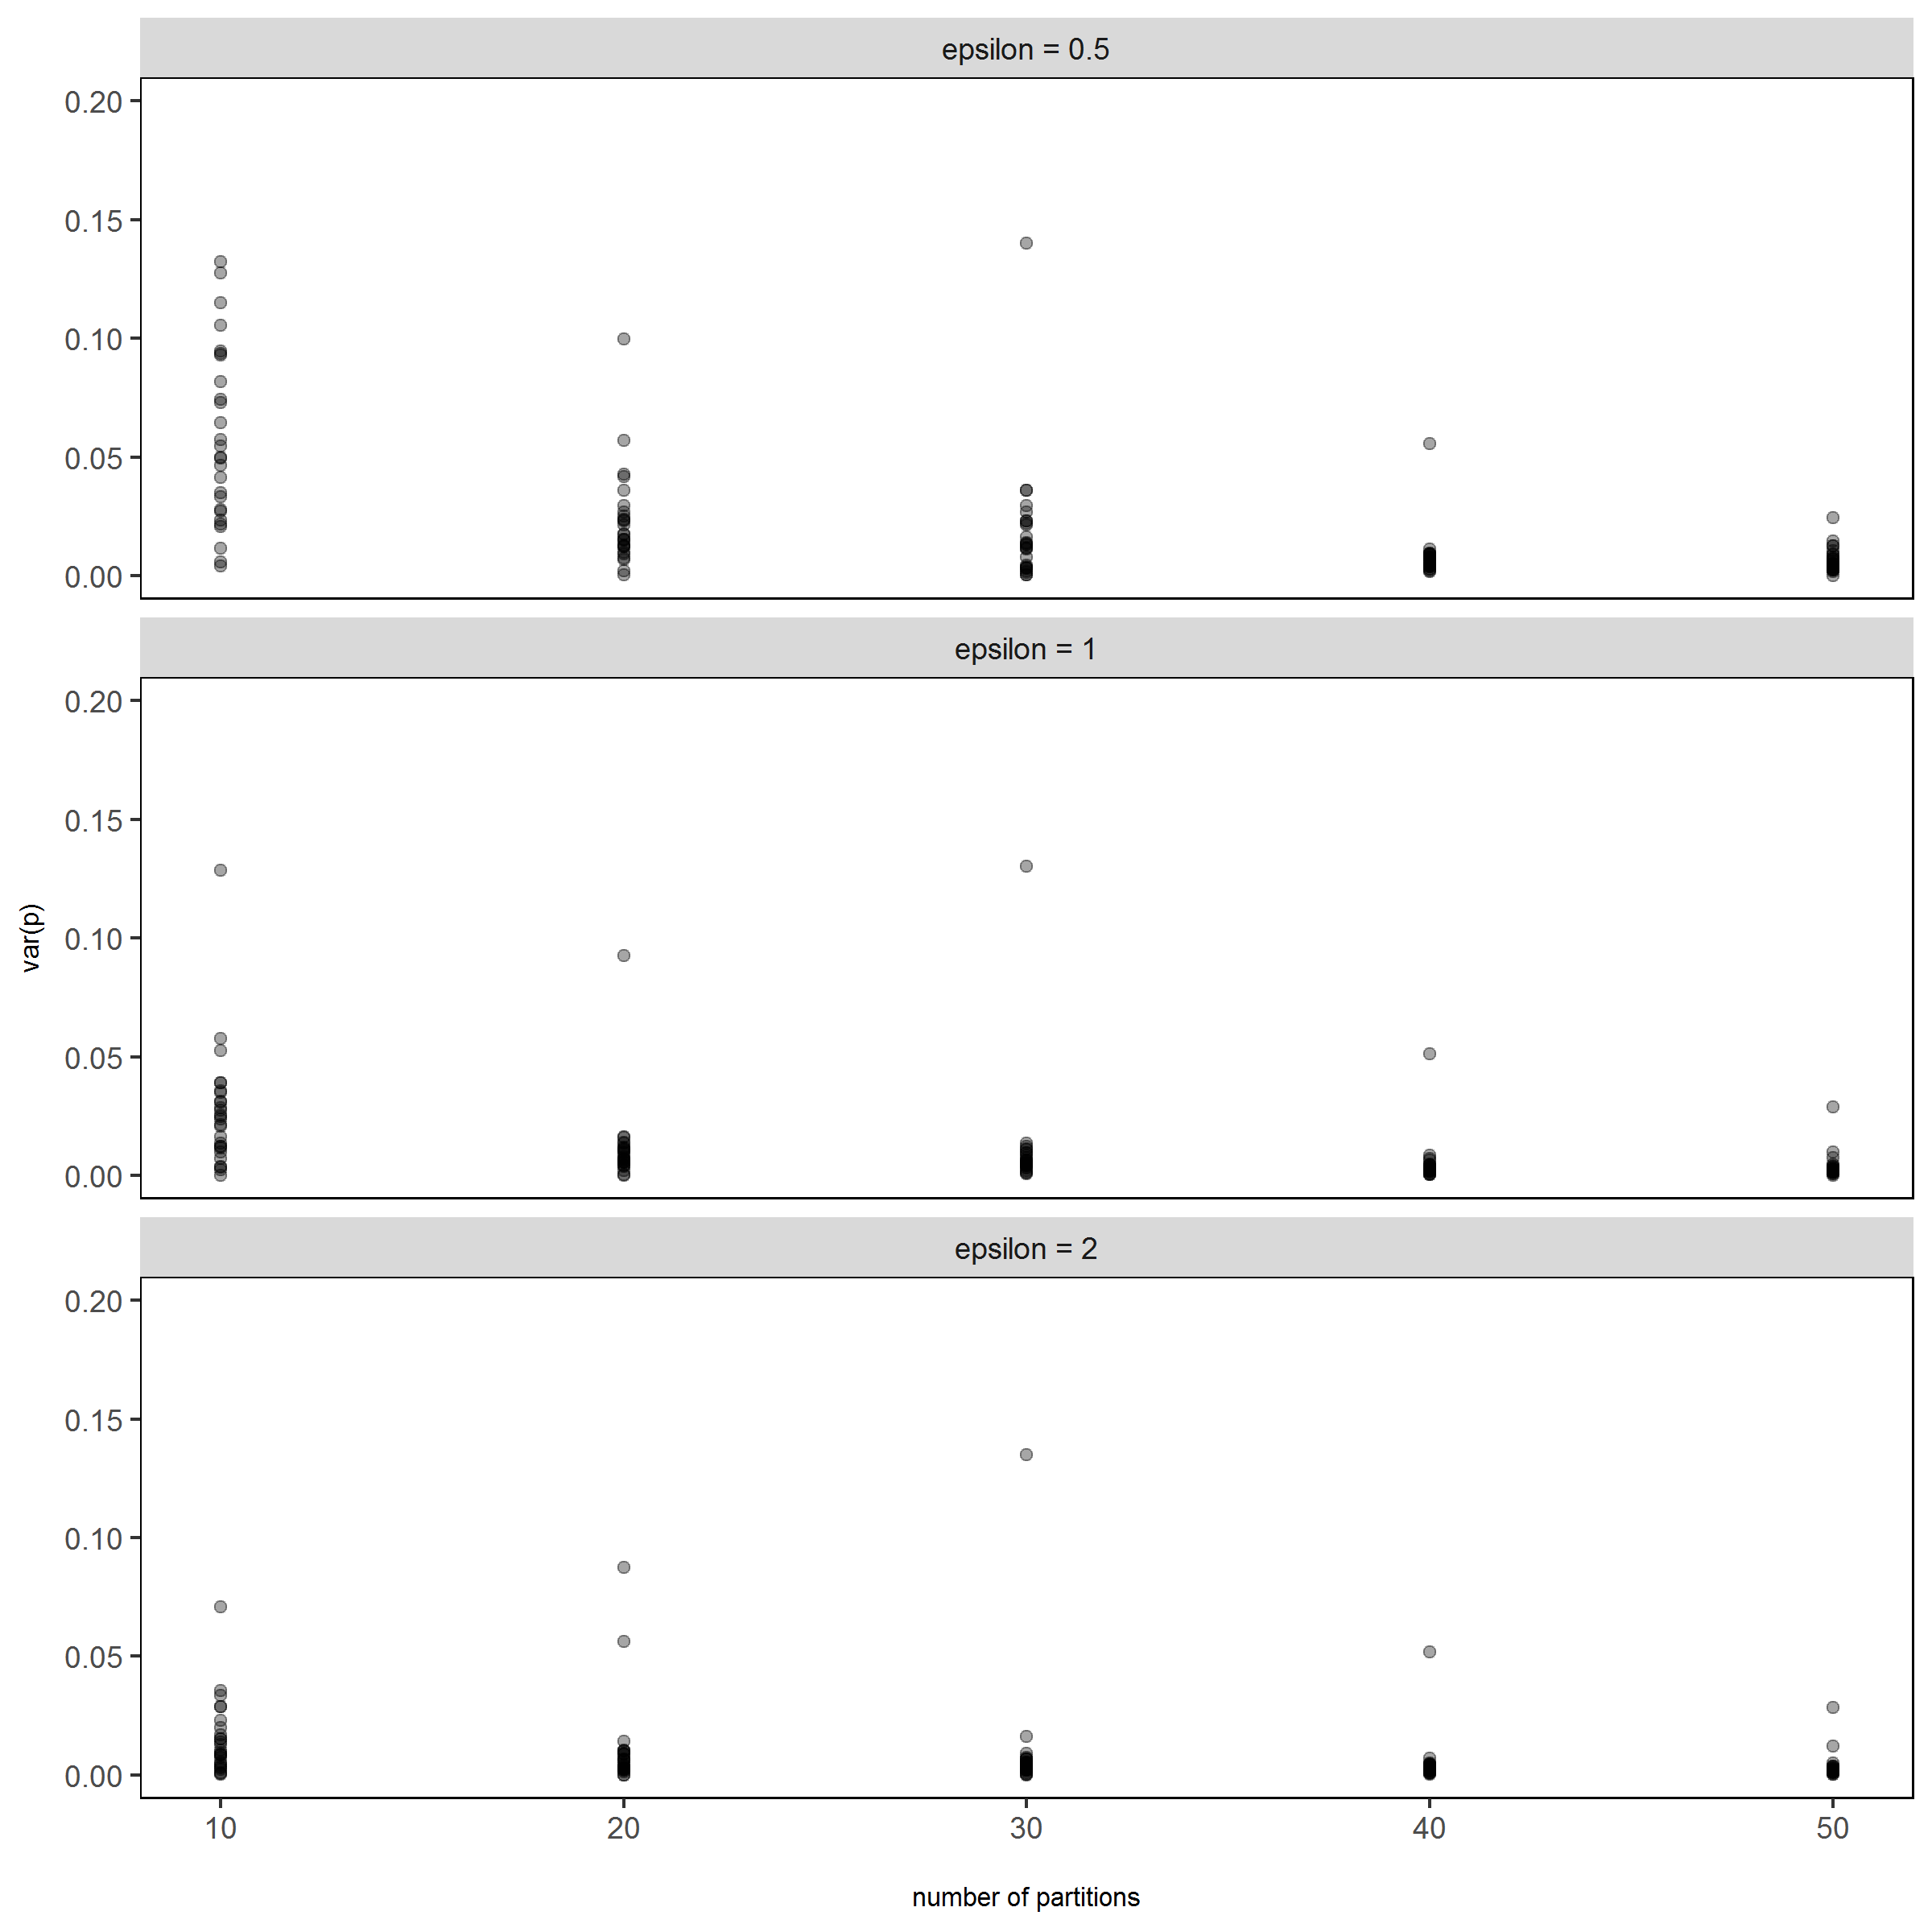
\includegraphics[width=6in]{RacePayDifferential-p-Variance-nPartitions.png}
    \caption{Variance of posterior p values with respect to M.  Each point represents the variance of ten posterior p values, from the ten iterations for each agency, occupation, sex, race, M, and $\epsilon$.}
    \label{figure:RacePayDifferential-p-Variance-nPartitions}
\end{figure}

\clearpage


\begin{figure}[h!]
    \centering
    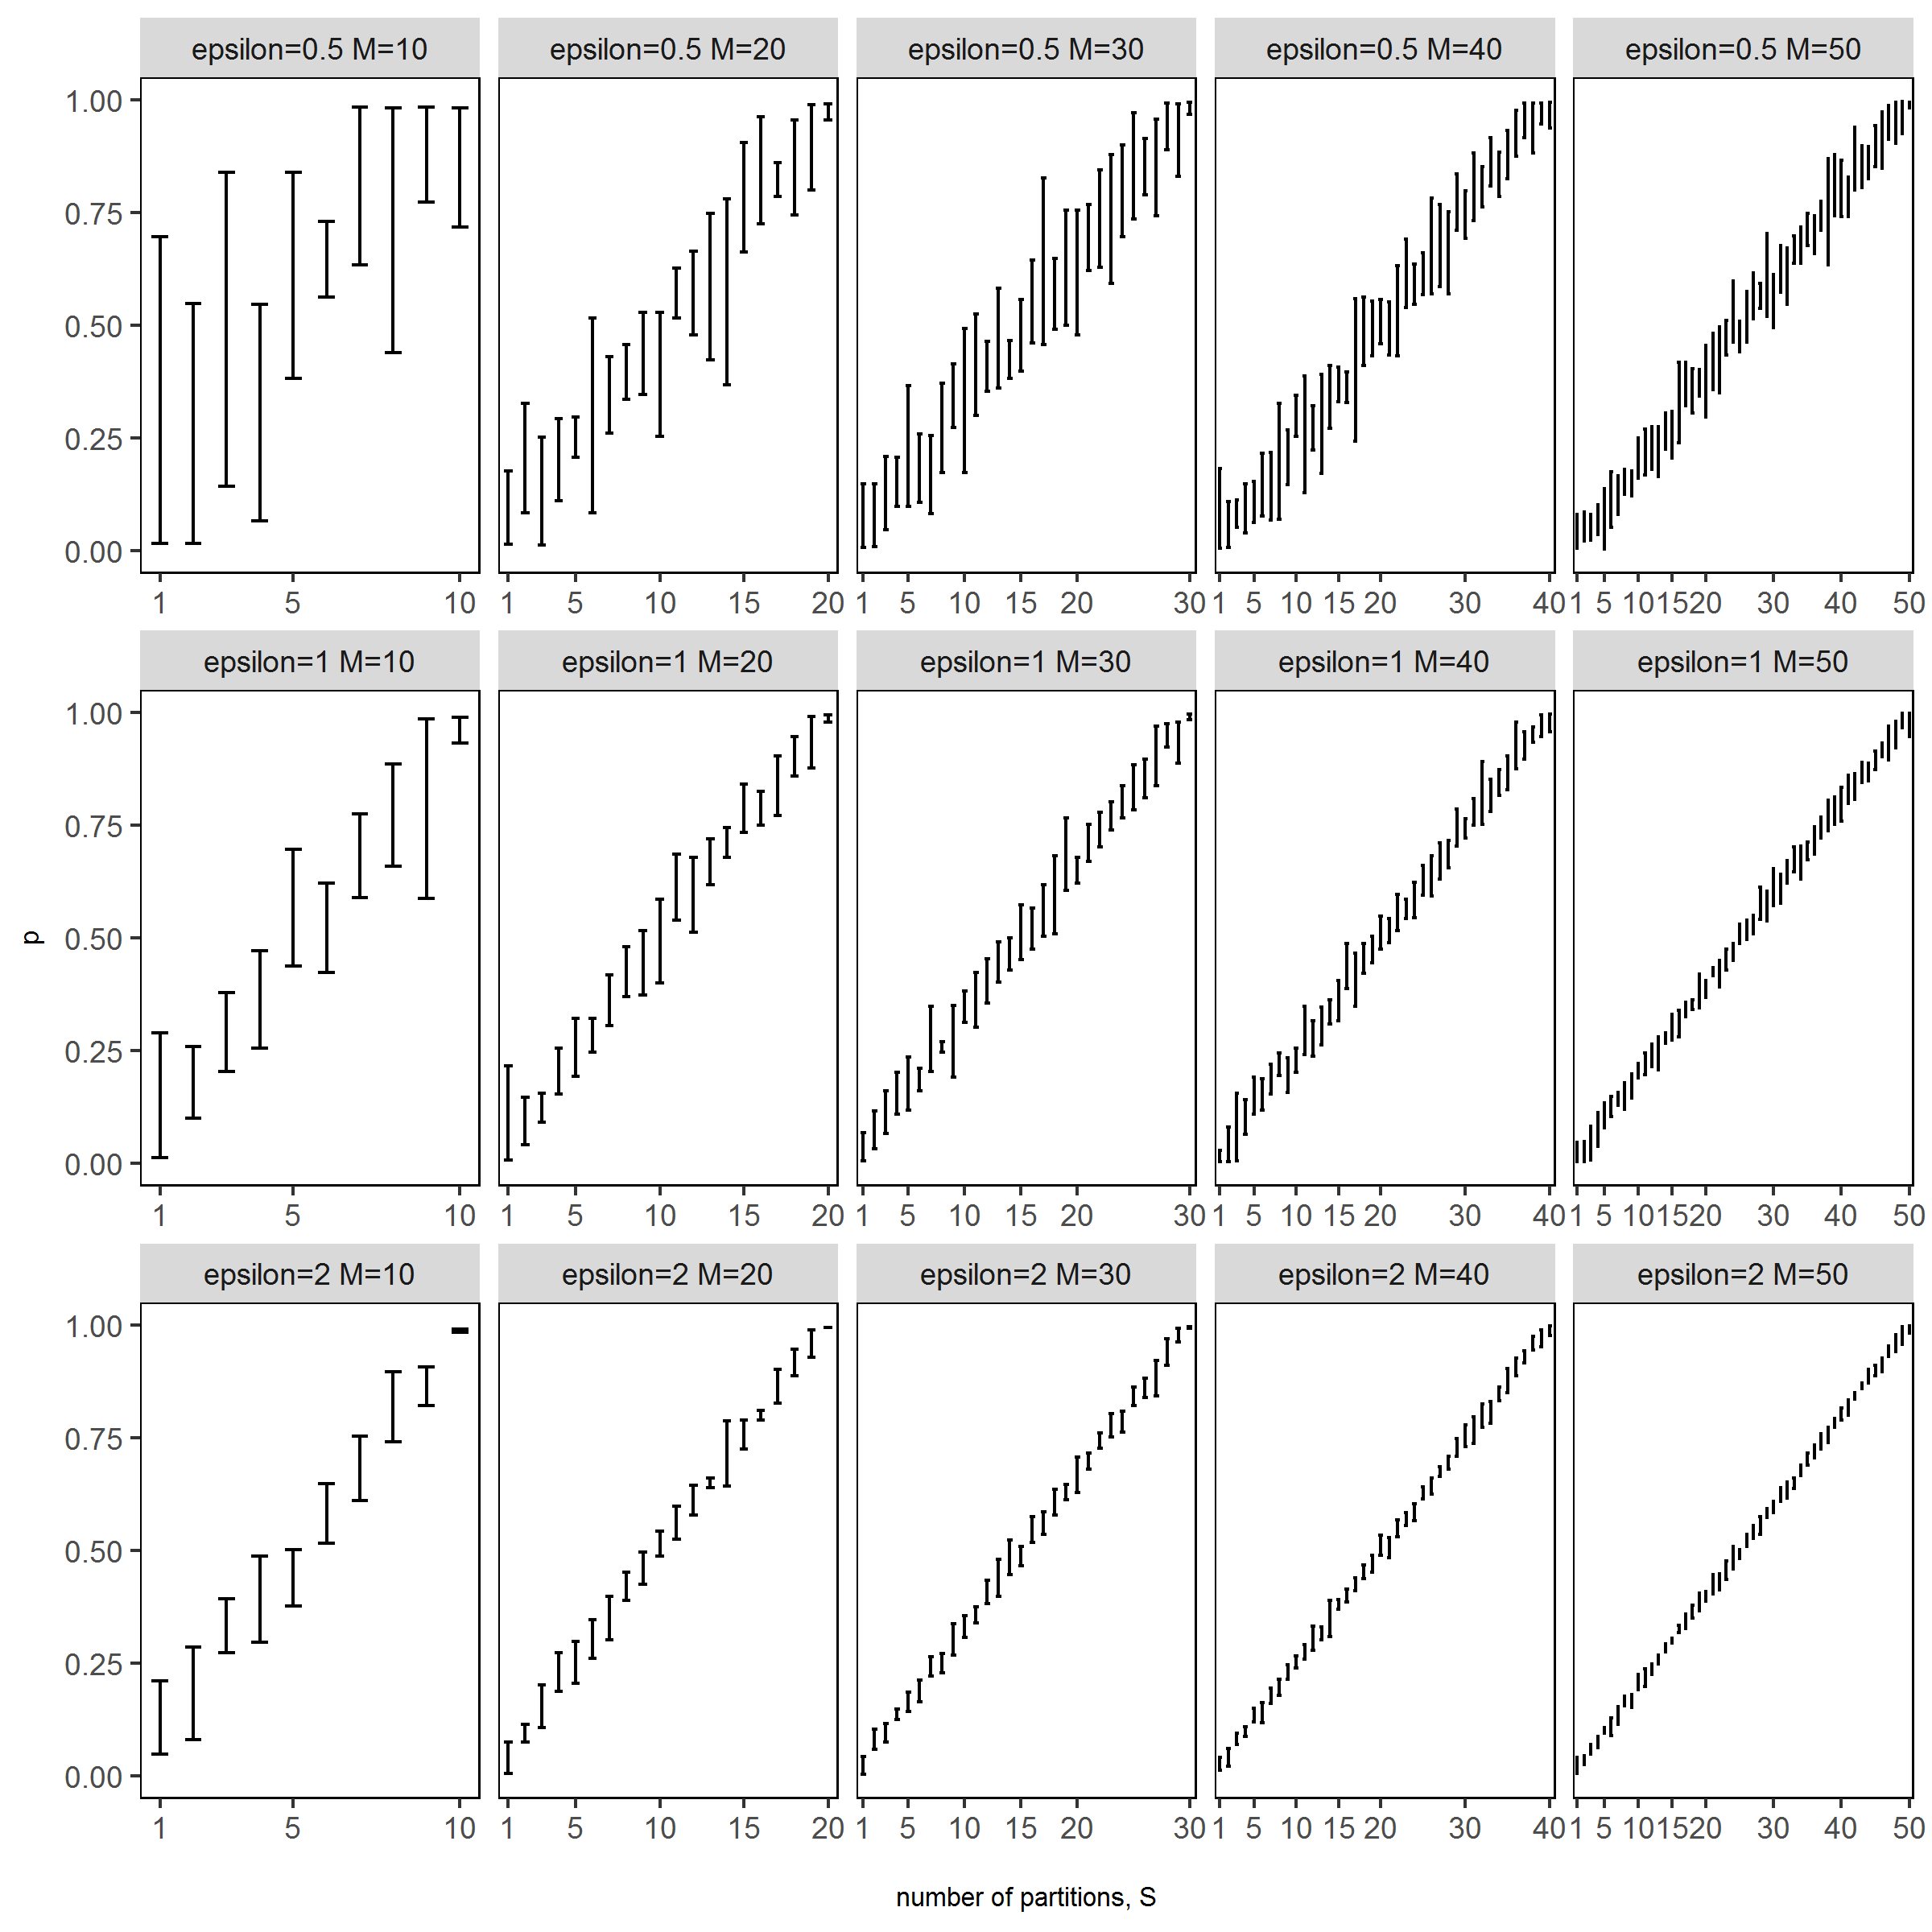
\includegraphics[width=6in]{RacePayDifferential-p-Simulation-10-90-Quantiles.png}
    \caption{10-90 percentile ranges of simulated posterior p values for indicated values of M and $\epsilon$.  Number of partitions at threshold, S, on x-axis.  Decrease in dispersion apparent with increase in M and $\epsilon$.}
    \label{figure:RacePayDifferential-p-Simulation-10-90-Quantiles}
\end{figure}

\clearpage

\end{spacing}
  
\end{document}